\documentclass{article}
%DIF LATEXDIFF DIFFERENCE FILE
%DIF DEL /tmp/r3_old.tex   Mon Sep 21 15:23:08 2026
%DIF ADD /tmp/r3_new.tex   Mon Sep 21 15:23:09 2026

\usepackage[T1]{fontenc}
\usepackage{iclr2027_conference,times}
%%%%% NEW MATH DEFINITIONS %%%%%

\usepackage{amsmath,amsfonts,bm}

% Mark sections of captions for referring to divisions of figures
\newcommand{\figleft}{{\em (Left)}}
\newcommand{\figcenter}{{\em (Center)}}
\newcommand{\figright}{{\em (Right)}}
\newcommand{\figtop}{{\em (Top)}}
\newcommand{\figbottom}{{\em (Bottom)}}
\newcommand{\captiona}{{\em (a)}}
\newcommand{\captionb}{{\em (b)}}
\newcommand{\captionc}{{\em (c)}}
\newcommand{\captiond}{{\em (d)}}

% Highlight a newly defined term
\newcommand{\newterm}[1]{{\bf #1}}


% Figure reference, lower-case.
\def\figref#1{figure~\ref{#1}}
% Figure reference, capital. For start of sentence
\def\Figref#1{Figure~\ref{#1}}
\def\twofigref#1#2{figures \ref{#1} and \ref{#2}}
\def\quadfigref#1#2#3#4{figures \ref{#1}, \ref{#2}, \ref{#3} and \ref{#4}}
% Section reference, lower-case.
\def\secref#1{section~\ref{#1}}
% Section reference, capital.
\def\Secref#1{Section~\ref{#1}}
% Reference to two sections.
\def\twosecrefs#1#2{sections \ref{#1} and \ref{#2}}
% Reference to three sections.
\def\secrefs#1#2#3{sections \ref{#1}, \ref{#2} and \ref{#3}}
% Reference to an equation, lower-case.
\def\eqref#1{equation~\ref{#1}}
% Reference to an equation, upper case
\def\Eqref#1{Equation~\ref{#1}}
% A raw reference to an equation---avoid using if possible
\def\plaineqref#1{\ref{#1}}
% Reference to a chapter, lower-case.
\def\chapref#1{chapter~\ref{#1}}
% Reference to an equation, upper case.
\def\Chapref#1{Chapter~\ref{#1}}
% Reference to a range of chapters
\def\rangechapref#1#2{chapters\ref{#1}--\ref{#2}}
% Reference to an algorithm, lower-case.
\def\algref#1{algorithm~\ref{#1}}
% Reference to an algorithm, upper case.
\def\Algref#1{Algorithm~\ref{#1}}
\def\twoalgref#1#2{algorithms \ref{#1} and \ref{#2}}
\def\Twoalgref#1#2{Algorithms \ref{#1} and \ref{#2}}
% Reference to a part, lower case
\def\partref#1{part~\ref{#1}}
% Reference to a part, upper case
\def\Partref#1{Part~\ref{#1}}
\def\twopartref#1#2{parts \ref{#1} and \ref{#2}}

\def\ceil#1{\lceil #1 \rceil}
\def\floor#1{\lfloor #1 \rfloor}
\def\1{\bm{1}}
\newcommand{\train}{\mathcal{D}}
\newcommand{\valid}{\mathcal{D_{\mathrm{valid}}}}
\newcommand{\test}{\mathcal{D_{\mathrm{test}}}}

\def\eps{{\epsilon}}


% Random variables
\def\reta{{\textnormal{$\eta$}}}
\def\ra{{\textnormal{a}}}
\def\rb{{\textnormal{b}}}
\def\rc{{\textnormal{c}}}
\def\rd{{\textnormal{d}}}
\def\re{{\textnormal{e}}}
\def\rf{{\textnormal{f}}}
\def\rg{{\textnormal{g}}}
\def\rh{{\textnormal{h}}}
\def\ri{{\textnormal{i}}}
\def\rj{{\textnormal{j}}}
\def\rk{{\textnormal{k}}}
\def\rl{{\textnormal{l}}}
% rm is already a command, just don't name any random variables m
\def\rn{{\textnormal{n}}}
\def\ro{{\textnormal{o}}}
\def\rp{{\textnormal{p}}}
\def\rq{{\textnormal{q}}}
\def\rr{{\textnormal{r}}}
\def\rs{{\textnormal{s}}}
\def\rt{{\textnormal{t}}}
\def\ru{{\textnormal{u}}}
\def\rv{{\textnormal{v}}}
\def\rw{{\textnormal{w}}}
\def\rx{{\textnormal{x}}}
\def\ry{{\textnormal{y}}}
\def\rz{{\textnormal{z}}}

% Random vectors
\def\rvepsilon{{\mathbf{\epsilon}}}
\def\rvtheta{{\mathbf{\theta}}}
\def\rva{{\mathbf{a}}}
\def\rvb{{\mathbf{b}}}
\def\rvc{{\mathbf{c}}}
\def\rvd{{\mathbf{d}}}
\def\rve{{\mathbf{e}}}
\def\rvf{{\mathbf{f}}}
\def\rvg{{\mathbf{g}}}
\def\rvh{{\mathbf{h}}}
\def\rvu{{\mathbf{i}}}
\def\rvj{{\mathbf{j}}}
\def\rvk{{\mathbf{k}}}
\def\rvl{{\mathbf{l}}}
\def\rvm{{\mathbf{m}}}
\def\rvn{{\mathbf{n}}}
\def\rvo{{\mathbf{o}}}
\def\rvp{{\mathbf{p}}}
\def\rvq{{\mathbf{q}}}
\def\rvr{{\mathbf{r}}}
\def\rvs{{\mathbf{s}}}
\def\rvt{{\mathbf{t}}}
\def\rvu{{\mathbf{u}}}
\def\rvv{{\mathbf{v}}}
\def\rvw{{\mathbf{w}}}
\def\rvx{{\mathbf{x}}}
\def\rvy{{\mathbf{y}}}
\def\rvz{{\mathbf{z}}}

% Elements of random vectors
\def\erva{{\textnormal{a}}}
\def\ervb{{\textnormal{b}}}
\def\ervc{{\textnormal{c}}}
\def\ervd{{\textnormal{d}}}
\def\erve{{\textnormal{e}}}
\def\ervf{{\textnormal{f}}}
\def\ervg{{\textnormal{g}}}
\def\ervh{{\textnormal{h}}}
\def\ervi{{\textnormal{i}}}
\def\ervj{{\textnormal{j}}}
\def\ervk{{\textnormal{k}}}
\def\ervl{{\textnormal{l}}}
\def\ervm{{\textnormal{m}}}
\def\ervn{{\textnormal{n}}}
\def\ervo{{\textnormal{o}}}
\def\ervp{{\textnormal{p}}}
\def\ervq{{\textnormal{q}}}
\def\ervr{{\textnormal{r}}}
\def\ervs{{\textnormal{s}}}
\def\ervt{{\textnormal{t}}}
\def\ervu{{\textnormal{u}}}
\def\ervv{{\textnormal{v}}}
\def\ervw{{\textnormal{w}}}
\def\ervx{{\textnormal{x}}}
\def\ervy{{\textnormal{y}}}
\def\ervz{{\textnormal{z}}}

% Random matrices
\def\rmA{{\mathbf{A}}}
\def\rmB{{\mathbf{B}}}
\def\rmC{{\mathbf{C}}}
\def\rmD{{\mathbf{D}}}
\def\rmE{{\mathbf{E}}}
\def\rmF{{\mathbf{F}}}
\def\rmG{{\mathbf{G}}}
\def\rmH{{\mathbf{H}}}
\def\rmI{{\mathbf{I}}}
\def\rmJ{{\mathbf{J}}}
\def\rmK{{\mathbf{K}}}
\def\rmL{{\mathbf{L}}}
\def\rmM{{\mathbf{M}}}
\def\rmN{{\mathbf{N}}}
\def\rmO{{\mathbf{O}}}
\def\rmP{{\mathbf{P}}}
\def\rmQ{{\mathbf{Q}}}
\def\rmR{{\mathbf{R}}}
\def\rmS{{\mathbf{S}}}
\def\rmT{{\mathbf{T}}}
\def\rmU{{\mathbf{U}}}
\def\rmV{{\mathbf{V}}}
\def\rmW{{\mathbf{W}}}
\def\rmX{{\mathbf{X}}}
\def\rmY{{\mathbf{Y}}}
\def\rmZ{{\mathbf{Z}}}

% Elements of random matrices
\def\ermA{{\textnormal{A}}}
\def\ermB{{\textnormal{B}}}
\def\ermC{{\textnormal{C}}}
\def\ermD{{\textnormal{D}}}
\def\ermE{{\textnormal{E}}}
\def\ermF{{\textnormal{F}}}
\def\ermG{{\textnormal{G}}}
\def\ermH{{\textnormal{H}}}
\def\ermI{{\textnormal{I}}}
\def\ermJ{{\textnormal{J}}}
\def\ermK{{\textnormal{K}}}
\def\ermL{{\textnormal{L}}}
\def\ermM{{\textnormal{M}}}
\def\ermN{{\textnormal{N}}}
\def\ermO{{\textnormal{O}}}
\def\ermP{{\textnormal{P}}}
\def\ermQ{{\textnormal{Q}}}
\def\ermR{{\textnormal{R}}}
\def\ermS{{\textnormal{S}}}
\def\ermT{{\textnormal{T}}}
\def\ermU{{\textnormal{U}}}
\def\ermV{{\textnormal{V}}}
\def\ermW{{\textnormal{W}}}
\def\ermX{{\textnormal{X}}}
\def\ermY{{\textnormal{Y}}}
\def\ermZ{{\textnormal{Z}}}

% Vectors
\def\vzero{{\bm{0}}}
\def\vone{{\bm{1}}}
\def\vmu{{\bm{\mu}}}
\def\vtheta{{\bm{\theta}}}
\def\va{{\bm{a}}}
\def\vb{{\bm{b}}}
\def\vc{{\bm{c}}}
\def\vd{{\bm{d}}}
\def\ve{{\bm{e}}}
\def\vf{{\bm{f}}}
\def\vg{{\bm{g}}}
\def\vh{{\bm{h}}}
\def\vi{{\bm{i}}}
\def\vj{{\bm{j}}}
\def\vk{{\bm{k}}}
\def\vl{{\bm{l}}}
\def\vm{{\bm{m}}}
\def\vn{{\bm{n}}}
\def\vo{{\bm{o}}}
\def\vp{{\bm{p}}}
\def\vq{{\bm{q}}}
\def\vr{{\bm{r}}}
\def\vs{{\bm{s}}}
\def\vt{{\bm{t}}}
\def\vu{{\bm{u}}}
\def\vv{{\bm{v}}}
\def\vw{{\bm{w}}}
\def\vx{{\bm{x}}}
\def\vy{{\bm{y}}}
\def\vz{{\bm{z}}}

% Elements of vectors
\def\evalpha{{\alpha}}
\def\evbeta{{\beta}}
\def\evepsilon{{\epsilon}}
\def\evlambda{{\lambda}}
\def\evomega{{\omega}}
\def\evmu{{\mu}}
\def\evpsi{{\psi}}
\def\evsigma{{\sigma}}
\def\evtheta{{\theta}}
\def\eva{{a}}
\def\evb{{b}}
\def\evc{{c}}
\def\evd{{d}}
\def\eve{{e}}
\def\evf{{f}}
\def\evg{{g}}
\def\evh{{h}}
\def\evi{{i}}
\def\evj{{j}}
\def\evk{{k}}
\def\evl{{l}}
\def\evm{{m}}
\def\evn{{n}}
\def\evo{{o}}
\def\evp{{p}}
\def\evq{{q}}
\def\evr{{r}}
\def\evs{{s}}
\def\evt{{t}}
\def\evu{{u}}
\def\evv{{v}}
\def\evw{{w}}
\def\evx{{x}}
\def\evy{{y}}
\def\evz{{z}}

% Matrix
\def\mA{{\bm{A}}}
\def\mB{{\bm{B}}}
\def\mC{{\bm{C}}}
\def\mD{{\bm{D}}}
\def\mE{{\bm{E}}}
\def\mF{{\bm{F}}}
\def\mG{{\bm{G}}}
\def\mH{{\bm{H}}}
\def\mI{{\bm{I}}}
\def\mJ{{\bm{J}}}
\def\mK{{\bm{K}}}
\def\mL{{\bm{L}}}
\def\mM{{\bm{M}}}
\def\mN{{\bm{N}}}
\def\mO{{\bm{O}}}
\def\mP{{\bm{P}}}
\def\mQ{{\bm{Q}}}
\def\mR{{\bm{R}}}
\def\mS{{\bm{S}}}
\def\mT{{\bm{T}}}
\def\mU{{\bm{U}}}
\def\mV{{\bm{V}}}
\def\mW{{\bm{W}}}
\def\mX{{\bm{X}}}
\def\mY{{\bm{Y}}}
\def\mZ{{\bm{Z}}}
\def\mBeta{{\bm{\beta}}}
\def\mPhi{{\bm{\Phi}}}
\def\mLambda{{\bm{\Lambda}}}
\def\mSigma{{\bm{\Sigma}}}

% Tensor
\DeclareMathAlphabet{\mathsfit}{\encodingdefault}{\sfdefault}{m}{sl}
\SetMathAlphabet{\mathsfit}{bold}{\encodingdefault}{\sfdefault}{bx}{n}
\newcommand{\tens}[1]{\bm{\mathsfit{#1}}}
\def\tA{{\tens{A}}}
\def\tB{{\tens{B}}}
\def\tC{{\tens{C}}}
\def\tD{{\tens{D}}}
\def\tE{{\tens{E}}}
\def\tF{{\tens{F}}}
\def\tG{{\tens{G}}}
\def\tH{{\tens{H}}}
\def\tI{{\tens{I}}}
\def\tJ{{\tens{J}}}
\def\tK{{\tens{K}}}
\def\tL{{\tens{L}}}
\def\tM{{\tens{M}}}
\def\tN{{\tens{N}}}
\def\tO{{\tens{O}}}
\def\tP{{\tens{P}}}
\def\tQ{{\tens{Q}}}
\def\tR{{\tens{R}}}
\def\tS{{\tens{S}}}
\def\tT{{\tens{T}}}
\def\tU{{\tens{U}}}
\def\tV{{\tens{V}}}
\def\tW{{\tens{W}}}
\def\tX{{\tens{X}}}
\def\tY{{\tens{Y}}}
\def\tZ{{\tens{Z}}}


% Graph
\def\gA{{\mathcal{A}}}
\def\gB{{\mathcal{B}}}
\def\gC{{\mathcal{C}}}
\def\gD{{\mathcal{D}}}
\def\gE{{\mathcal{E}}}
\def\gF{{\mathcal{F}}}
\def\gG{{\mathcal{G}}}
\def\gH{{\mathcal{H}}}
\def\gI{{\mathcal{I}}}
\def\gJ{{\mathcal{J}}}
\def\gK{{\mathcal{K}}}
\def\gL{{\mathcal{L}}}
\def\gM{{\mathcal{M}}}
\def\gN{{\mathcal{N}}}
\def\gO{{\mathcal{O}}}
\def\gP{{\mathcal{P}}}
\def\gQ{{\mathcal{Q}}}
\def\gR{{\mathcal{R}}}
\def\gS{{\mathcal{S}}}
\def\gT{{\mathcal{T}}}
\def\gU{{\mathcal{U}}}
\def\gV{{\mathcal{V}}}
\def\gW{{\mathcal{W}}}
\def\gX{{\mathcal{X}}}
\def\gY{{\mathcal{Y}}}
\def\gZ{{\mathcal{Z}}}

% Sets
\def\sA{{\mathbb{A}}}
\def\sB{{\mathbb{B}}}
\def\sC{{\mathbb{C}}}
\def\sD{{\mathbb{D}}}
% Don't use a set called E, because this would be the same as our symbol
% for expectation.
\def\sF{{\mathbb{F}}}
\def\sG{{\mathbb{G}}}
\def\sH{{\mathbb{H}}}
\def\sI{{\mathbb{I}}}
\def\sJ{{\mathbb{J}}}
\def\sK{{\mathbb{K}}}
\def\sL{{\mathbb{L}}}
\def\sM{{\mathbb{M}}}
\def\sN{{\mathbb{N}}}
\def\sO{{\mathbb{O}}}
\def\sP{{\mathbb{P}}}
\def\sQ{{\mathbb{Q}}}
\def\sR{{\mathbb{R}}}
\def\sS{{\mathbb{S}}}
\def\sT{{\mathbb{T}}}
\def\sU{{\mathbb{U}}}
\def\sV{{\mathbb{V}}}
\def\sW{{\mathbb{W}}}
\def\sX{{\mathbb{X}}}
\def\sY{{\mathbb{Y}}}
\def\sZ{{\mathbb{Z}}}

% Entries of a matrix
\def\emLambda{{\Lambda}}
\def\emA{{A}}
\def\emB{{B}}
\def\emC{{C}}
\def\emD{{D}}
\def\emE{{E}}
\def\emF{{F}}
\def\emG{{G}}
\def\emH{{H}}
\def\emI{{I}}
\def\emJ{{J}}
\def\emK{{K}}
\def\emL{{L}}
\def\emM{{M}}
\def\emN{{N}}
\def\emO{{O}}
\def\emP{{P}}
\def\emQ{{Q}}
\def\emR{{R}}
\def\emS{{S}}
\def\emT{{T}}
\def\emU{{U}}
\def\emV{{V}}
\def\emW{{W}}
\def\emX{{X}}
\def\emY{{Y}}
\def\emZ{{Z}}
\def\emSigma{{\Sigma}}

% entries of a tensor
% Same font as tensor, without \bm wrapper
\newcommand{\etens}[1]{\mathsfit{#1}}
\def\etLambda{{\etens{\Lambda}}}
\def\etA{{\etens{A}}}
\def\etB{{\etens{B}}}
\def\etC{{\etens{C}}}
\def\etD{{\etens{D}}}
\def\etE{{\etens{E}}}
\def\etF{{\etens{F}}}
\def\etG{{\etens{G}}}
\def\etH{{\etens{H}}}
\def\etI{{\etens{I}}}
\def\etJ{{\etens{J}}}
\def\etK{{\etens{K}}}
\def\etL{{\etens{L}}}
\def\etM{{\etens{M}}}
\def\etN{{\etens{N}}}
\def\etO{{\etens{O}}}
\def\etP{{\etens{P}}}
\def\etQ{{\etens{Q}}}
\def\etR{{\etens{R}}}
\def\etS{{\etens{S}}}
\def\etT{{\etens{T}}}
\def\etU{{\etens{U}}}
\def\etV{{\etens{V}}}
\def\etW{{\etens{W}}}
\def\etX{{\etens{X}}}
\def\etY{{\etens{Y}}}
\def\etZ{{\etens{Z}}}

% The true underlying data generating distribution
\newcommand{\pdata}{p_{\rm{data}}}
% The empirical distribution defined by the training set
\newcommand{\ptrain}{\hat{p}_{\rm{data}}}
\newcommand{\Ptrain}{\hat{P}_{\rm{data}}}
% The model distribution
\newcommand{\pmodel}{p_{\rm{model}}}
\newcommand{\Pmodel}{P_{\rm{model}}}
\newcommand{\ptildemodel}{\tilde{p}_{\rm{model}}}
% Stochastic autoencoder distributions
\newcommand{\pencode}{p_{\rm{encoder}}}
\newcommand{\pdecode}{p_{\rm{decoder}}}
\newcommand{\precons}{p_{\rm{reconstruct}}}

\newcommand{\laplace}{\mathrm{Laplace}} % Laplace distribution

\newcommand{\E}{\mathbb{E}}
\newcommand{\Ls}{\mathcal{L}}
\newcommand{\R}{\mathbb{R}}
\newcommand{\emp}{\tilde{p}}
\newcommand{\lr}{\alpha}
\newcommand{\reg}{\lambda}
\newcommand{\rect}{\mathrm{rectifier}}
\newcommand{\softmax}{\mathrm{softmax}}
\newcommand{\sigmoid}{\sigma}
\newcommand{\softplus}{\zeta}
\newcommand{\KL}{D_{\mathrm{KL}}}
\newcommand{\Var}{\mathrm{Var}}
\newcommand{\standarderror}{\mathrm{SE}}
\newcommand{\Cov}{\mathrm{Cov}}
% Wolfram Mathworld says $L^2$ is for function spaces and $\ell^2$ is for vectors
% But then they seem to use $L^2$ for vectors throughout the site, and so does
% wikipedia.
\newcommand{\normlzero}{L^0}
\newcommand{\normlone}{L^1}
\newcommand{\normltwo}{L^2}
\newcommand{\normlp}{L^p}
\newcommand{\normmax}{L^\infty}

\newcommand{\parents}{Pa} % See usage in notation.tex. Chosen to match Daphne's book.

\DeclareMathOperator*{\argmax}{arg\,max}
\DeclareMathOperator*{\argmin}{arg\,min}

\DeclareMathOperator{\sign}{sign}
\DeclareMathOperator{\Tr}{Tr}
\let\ab\allowbreak


\usepackage{float}
\usepackage{hyperref}
\usepackage{url}
\usepackage{graphicx}
\usepackage{amsmath,amssymb,bm}
\usepackage{booktabs,array,multirow,threeparttable,adjustbox}
\usepackage{placeins}
\usepackage{tikz}
\usetikzlibrary{arrows.meta,positioning,fit,calc}
\hypersetup{hidelinks,hypertexnames=false}

\title{RAL-MoE-ROM: Hierarchical Mixture-of-Experts for Regime-Adaptive Reduced-Order Model }

% Anonymous submission. Restore the author block only for the camera-ready version.
\author{Anonymous Authors}

% Keep disabled for the anonymous submission.
% \iclrfinalcopy

% Non-destructive TeX annotation layer. Scientific pixels, legends and
% numerical error annotations remain in the original archived PNGs.
\newcommand{\FieldPanel}[2]{%
\begin{tikzpicture}
\node[anchor=south west,inner sep=0] (im) at (0,0)
 {\includegraphics[width=0.80\linewidth]{#1}};
\begin{scope}[x={(im.south east)},y={(im.north west)}]
 \fill[white] (0,0.13) rectangle (0.055,0.98);
 \node[rotate=90,font=\scriptsize\bfseries] at (0.023,0.863) {Reference};
 \node[rotate=90,font=\scriptsize\bfseries] at (0.023,0.656) {#2};
 \node[rotate=90,font=\scriptsize\bfseries] at (0.023,0.449) {Hopf};
 \node[rotate=90,font=\scriptsize\bfseries] at (0.023,0.242) {RAL-MoE-ROM};
\end{scope}
\end{tikzpicture}%
}
\newcommand{\ErrorPanel}[2]{%
\begin{tikzpicture}
\node[anchor=south west,inner sep=0] (im) at (0,0)
 {\includegraphics[width=0.80\linewidth]{#1}};
\begin{scope}[x={(im.south east)},y={(im.north west)}]
 \fill[white] (0,0.17) rectangle (0.055,0.985);
 \node[rotate=90,font=\scriptsize\bfseries] at (0.023,0.83) {#2};
 \node[rotate=90,font=\scriptsize\bfseries] at (0.023,0.57) {Hopf};
 \node[rotate=90,font=\scriptsize\bfseries] at (0.023,0.31) {RAL-MoE-ROM};
 \foreach \x/\y/\lab in {0.080/0.932/i,0.583/0.932/j,0.080/0.673/k,0.583/0.673/l,0.080/0.415/m,0.583/0.415/n}{
  \fill[white] (\x-0.018,\y-0.020) rectangle (\x+0.018,\y+0.020);
  \node[font=\scriptsize\bfseries,inner sep=0] at (\x,\y) {(\lab)};
 }
\end{scope}
\end{tikzpicture}%
}
%DIF PREAMBLE EXTENSION ADDED BY LATEXDIFF
%DIF CFONT PREAMBLE %DIF PREAMBLE
\RequirePackage{color}\definecolor{RED}{rgb}{1,0,0}\definecolor{BLUE}{rgb}{0,0,1} %DIF PREAMBLE
\DeclareOldFontCommand{\sf}{\normalfont\sffamily}{\mathsf} %DIF PREAMBLE
\providecommand{\DIFaddtex}[1]{{\protect\color{blue} \sf #1}} %DIF PREAMBLE
\providecommand{\DIFdeltex}[1]{{\protect\color{red} \scriptsize #1}} %DIF PREAMBLE
%DIF SAFE PREAMBLE %DIF PREAMBLE
\providecommand{\DIFaddbegin}{} %DIF PREAMBLE
\providecommand{\DIFaddend}{} %DIF PREAMBLE
\providecommand{\DIFdelbegin}{} %DIF PREAMBLE
\providecommand{\DIFdelend}{} %DIF PREAMBLE
\providecommand{\DIFmodbegin}{} %DIF PREAMBLE
\providecommand{\DIFmodend}{} %DIF PREAMBLE
%DIF FLOATSAFE PREAMBLE %DIF PREAMBLE
\providecommand{\DIFaddFL}[1]{\DIFadd{#1}} %DIF PREAMBLE
\providecommand{\DIFdelFL}[1]{\DIFdel{#1}} %DIF PREAMBLE
\providecommand{\DIFaddbeginFL}{} %DIF PREAMBLE
\providecommand{\DIFaddendFL}{} %DIF PREAMBLE
\providecommand{\DIFdelbeginFL}{} %DIF PREAMBLE
\providecommand{\DIFdelendFL}{} %DIF PREAMBLE
%DIF HYPERREF PREAMBLE %DIF PREAMBLE
\providecommand{\DIFadd}[1]{\texorpdfstring{\DIFaddtex{#1}}{#1}} %DIF PREAMBLE
\providecommand{\DIFdel}[1]{\texorpdfstring{\DIFdeltex{#1}}{}} %DIF PREAMBLE
%DIF END PREAMBLE EXTENSION ADDED BY LATEXDIFF

\begin{document}
\raggedbottom

\maketitle
\begin{center}\small Third batch versus first batch: {\color{blue}added}; {\color{red}deleted}. Tables, figures and equations are compared as complete blocks.\end{center}

\begin{abstract}
Reduced-order models (ROMs) approximate high-dimensional dynamical systems using a small number of state variables. However, their predictive accuracy can deteriorate when parameter changes lead to different dynamical regimes. Different regimes may require different reduced representations and dynamics, making it difficult for a single model to remain accurate across the full parameter range. We introduce RAL-MoE-ROM, a hierarchical mixture-of-experts framework with two levels: regime-local specialists and cross-regime routing with fusion.. At the first level, each local model, called a specialist, uses a structured sparse mixture of experts to improve its reduced dynamics and is trained through multi-step autonomous rollouts. At the second level, an outer router selects a specialist or a pair of neighboring specialists. When two specialists are selected, a learned gate uses the initial physical history to combine their reconstructed fields. Across three flow benchmarks spanning steady, Hopf-onset, and periodic regimes, the local specialists provide accurate autonomous predictions, while cross-regime routing further improve prediction in the evaluated regime overlaps.
\end{abstract}

\section{Introduction}

High-fidelity simulations of high-dimensional dynamical systems
can be expensive when repeated predictions are required across many parameter settings. Reduced-order models (ROMs) provide a cost-effective surrogate by representing the physical state with a small number of state variables. The problem becomes more challenging when changing a parameter also changes the type of regimes. In incompressible flows, for example, varying the Reynolds number can lead from relaxation toward a steady state to oscillatory growth and sustained periodic motion. A useful predictive model must capture these regimes while evolving autonomously.



Such regime variation introduces two closely related challenges for ROMs. The first concerns representation: spatial structures that are important in one regime may differ from those required in another, making a single representation less effective. The second is dynamical: the reduced evolution law must accommodate qualitatively different behaviors, including stable relaxation, instability growth, and nonlinear periodic oscillations. Increasing model capacity alone cannot compensate for an inadequate reduced representation, while improving the representation does not by itself guarantee accurate autonomous rollout. These observations motivate adapting the local representation and the local dynamics separately, while providing a consistent way to assemble their predictions.




Projection-based ROMs provide an explicit reduced representation and reduced dynamics, commonly through proper orthogonal decomposition (POD) and Galerkin projection \citep{sirovich1987,berkooz1993,benner2015}. However,projection-based ROMs are inherently affected by truncation, which neglects the influence of discarded modes on the retained coordinates, leading to closure errors that degrade long-horizon prediction.\citep{amsallem2012}. Data-driven ROMs offer greater flexibility in approximating nonlinear dynamics, but low one-step error does not guarantee accurate autonomous rollouts, and they often lack physical interpretability\citep{duraisamy2019,brunton2020}. Hybrid ROMs combine projection-based ROMs with learned corrections or learned reduced representations, retaining physical structure while increasing approximation flexibility
\citep{dar2023,lee2020,fresca2022,geelen2023}. These developments improve the modeling of reduced dynamics, but they do not by themselves resolve the representational difficulty that arises when qualitatively different regimes must be described over a broad parameter range.





A complementary strategy localizes the reduced representation, using multiple subspaces, clusters, or manifolds for different portions of the solution set \citep{kaiser2014,li2021cluster,diaz2024}. These directions address complementary aspects of the broad-parameter problem: hybrid modeling improves the fidelity of the reduced dynamics, whereas localization adapts the reduced representation to regime-dependent structures. Localization, however, creates a new assembly problem.  Independently constructed local ROMs generally have different reduced state variables and  operators, so their reduced coordinates are chart-specific. Direct interpolation or averaging in reduced-coordinate space therefore has no natural cross-chart interpretation. Mixture-of-experts (MoE) architectures provide a natural framework for conditional specialization \citep{jacobs1991,jordan1994,shazeer2017,fedus2022}, but standard MoE formulations typically route specialized predictors within a shared representation or common feature space. Here, in contrast, the experts are complete local ROMs whose coordinates are not shared. The problem is therefore not only routing among local ROMs, but also assembling or fusing their outputs across representations. This makes the problem hierarchical: one must adapt the reduced dynamics within each local representation and, separately, route to and fuse complete local ROMs across representations. This raises a distinct question that standard within-representation MoE routing does not address: how can independently constructed local dynamical models be routed and assembled without forcing them into a common latent coordinate system?


To address this gap, we introduce the Regime-Adaptive Localized Mixture-of-Experts Reduced-Order Model (RAL-MoE-ROM), a two-level hierarchical framework that separates regime-local reduced dynamics from cross-regime routing and fusion. The parameter domain is covered by prescribed, overlapping regime-local regions, each equipped with an independent  autonomous specialist. At the first level, each specialist, use an explicit projected-based ROM  and augments it with sparsely  structured MOEs which trained trained through  multi-step autonomous rollouts. Rather than using conventional MLP-only experts, each activated expert decomposes its output into three additive components: a nonlinear neural branch, together with explicit linear and low-rank quadratic branches derived from the projection-based. At the second level, a parameter-conditioned outer router produces window-level routing weights over the local specialists, while a fixed applicability mask determines whether inference uses one specialist or a pair of adjacent specialists. When two specialists are selected, a learned fusion gate combines their reconstructed physical fields conditioned on the initial physical history. The overall architecture is illustrated in Figure~\ref{fig:ral_overview}, highlighting the regime-local specialists and the cross-regime routing and fusion mechanism.




Our main contributions are as follows:
\begin{itemize}

\item \textbf{Structured regime-local specialists for autonomous reduced dynamics.} Each specialist combines a physics-based ROM with a structured sparse MoE closure and is trained under closed-loop multi-step rollouts.

\item \textbf{Cross-regime routing and fusion.}
An outer router selects a specialist or a pair of neighboring specialists. When two specialists are selected, a learned gate uses the initial physical history to combine their reconstructed fields.

\item \textbf{Multi-regime evaluation.}
We evaluate the framework on  incompressible-flow benchmarks spanning steady, Hopf-onset, and periodic regimes. The experiments assess autonomous specialist rollouts, cross-regime routing and fusion in regime overlaps, and the main local architectural choices, providing complementary evidence for the proposed local modeling and assembly strategy.

\end{itemize}




\par


\begin{figure}[t]
    \centering
    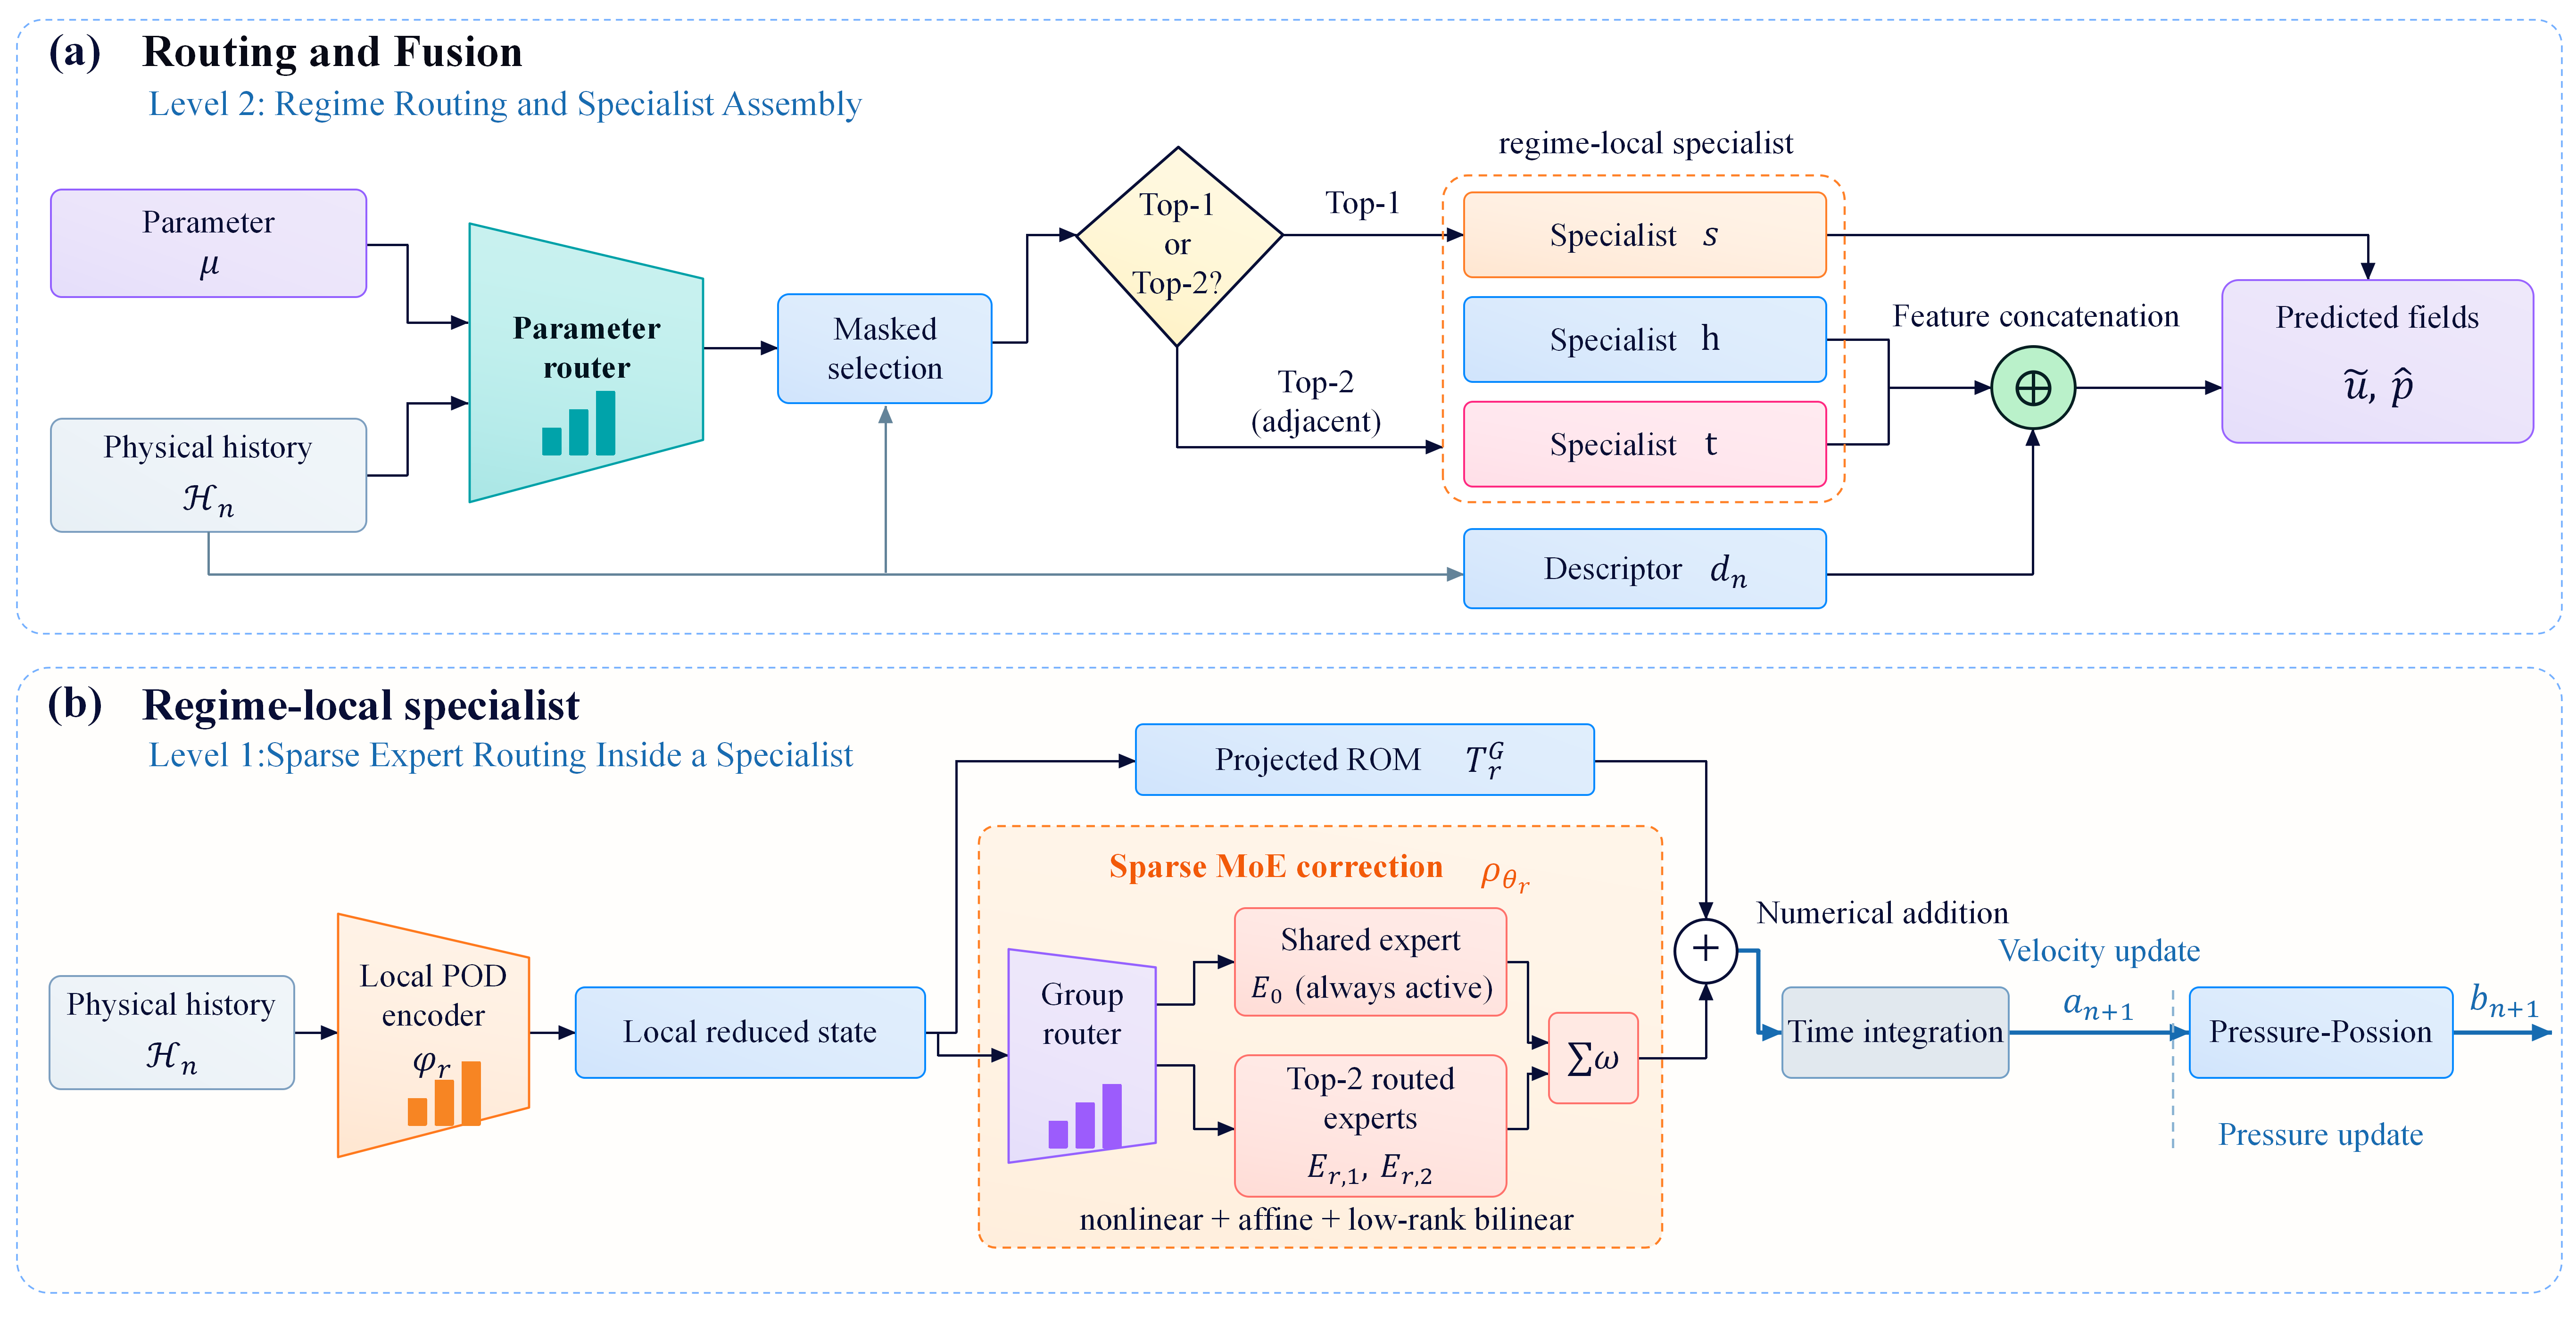
\includegraphics[width=\linewidth]{figures/flowchat.png}
\caption{
Overview of RAL-MoE-ROM.
(a) A parameter-only outer router provides trajectory-level preferences over regime-local specialists, while an applicability mask restricts inference to a single specialist or an adjacent pair. When an adjacent pair is used, a history-conditioned
gate combines only their reconstructed physical fields.
(b) Each regime-local specialist augments a projected ROMs  with a structured sparse MoE correction.
}
    \label{fig:ral_overview}
\end{figure}


\par



\section{Related Work}
\paragraph{Projection, learned dynamics, and autonomous rollout.}
POD--Galerkin methods project the governing equations onto a reduced basis and retain an explicit reduced dynamical system \citep{sirovich1987,berkooz1993,benner2015}. Their long-horizon accuracy can deteriorate when truncated interactions are not adequately represented, motivating closure and stabilization strategies
\citep{amsallem2012}. Non-intrusive and data-driven ROMs instead infer reduced evolution laws directly from simulation data, ranging from projection-based operator inference to neural and latent-state dynamics
\citep{peherstorfer2016,hesthaven2018,champion2019,lee2020, pan2024domain,park2024}. Operator-inference methods provide a particularly direct connection between data-driven reduced dynamics and classical projection-based ROMs \citep{peherstorfer2016}. Neural-operator approaches learn mappings between function spaces rather than explicit low-dimensional state evolution\citep{lu2021,kovachki2023}. Hybrid ROMs retain projected or physics-based structure while learning missing or unresolved reduced dynamics \citep{duraisamy2019,fresca2022,dar2023}. RAL-MoE-ROM follows this hybrid principle, but places a structured sparse-MoE correction inside each regime-local ROM and trains the resulting specialist under multi-step  autonomous rollout.



\paragraph{Localized representations and local reduced dynamics.}
Localization has been explored through parameter-dependent reduced bases, localized operators and nonlinear manifolds \citep{amsallem2008,peherstorfer2014,kaiser2014,li2021cluster,diaz2024,bhat2025}. These approaches all reduce the burden on a single global representation, differing in whether localization is performed along parameter, state, or spatial coordinates. Recent work has further emphasized explicitly local reduced dynamics. More recently, ql-ROM partitions the solution manifold into clusters, constructs an intrusive ROM within each cluster, and connects the local models through assignment and change-of-basis operations
\citep{colanera2025}. Therefore, when complete local ROMs are constructed independently, their reduced coordinates and operators need not be directly compatible, so switching or combining them requires an explicit coordination mechanism. RAL-MoE-ROM takes a different approach: instead of coordinating local models in reduced-coordinate space, it lets local specialists evolve independently in their native coordinates and combines neighboring predictions only after reconstruction in the common physical space.





\paragraph{Mixture-of-experts and cross-chart assembly.}
Classical hierarchical mixtures learn conditional expert assignments \citep{jacobs1991,jordan1994}, while sparse MoE architectures activate only a subset of experts for each input \citep{shazeer2017,fedus2022}. MoE-based conditional specialization has also been introduced into scientific machine learning, including physics-informed constraints, 
neural-operator pretraining, and PDE forecasting
\citep{ICLR2024_9aeda582,NEURIPS2024_b83fae17,
NEURIPS2025_2d23a999,ICLR2026_754612bd}. These methods demonstrate the value of conditional specialization, but do
not address routing among complete autonomous ROMs. RAL-MoE-ROM therefore applies router  at two levels: sparse experts model unresolved dynamics within each local ROM, while an outer router acts on the complete regime-local specialists. The outer level selects a single specialist or an
applicable neighboring pair, with the latter combined through a history-conditioned gate after physical reconstruction.



\section{RAL-MoE-ROM}
\label{sec:method}

RAL-MoE-ROM separates reduced modeling into three complementary components: regime-local ROMs, autonomous local specialists, and cross-regime router and fusion. These components are organized by a two-level routing hierarchy. 

\subsection{Overlapping regime-local reduced charts}

Let $r\in\{S,H,P\}$ index steady, Hopf-onset, and periodic regimes, and let $\mathcal M_r$ denote the corresponding overlapping parameter regions. Each regime-local parameter region is equipped with its own reduced coordinate system. A physical velocity field is encoded and reconstructed as


\begin{equation}
  \bm a^{(r)}={\Phi_u^{(r)}}^{\top}M_u(\bm u-\bar{\bm u}^{(r)}),\qquad
  \widehat{\bm u}^{(r)}=\bar{\bm u}^{(r)}+\Phi_u^{(r)}\bm a^{(r)},
  \label{eq:main_chart}
\end{equation}


where $M_u$ is the finite-volume quadrature matrix. Gauge-corrected pressure is encoded analogously, yielding local coefficients
$\bm b^{(r)}$. 

A reduced chart comprises its mean fields, velocity and pressure bases, local coordinates, and normalization statistics. Each chart is associated with a regime-local parameter region and its own projected operators.
These quantities are constructed independently across regimes. Even when two charts have the same reduced dimension, their coordinates are not assumed to be componentwise aligned. Cross-regime assembly is consequently performed only after reconstruction in physical space.

\subsection{Regime-local hybrid specialists}

For the additive hybrid instances, a projected Galerkin backbone describes the resolved dynamics, while a learned closure accounts for the unresolved reduced dynamics:


\begin{equation}
  \dot{\bm a}^{(r)}=
  \underbrace{\bm c_r+\bm A_r\bm a^{(r)}+
  \bm H_r:\bigl(\bm a^{(r)}\otimes\bm a^{(r)}\bigr)+
  \bm C^p_r\bm b^{(r)}}_{\mathcal F_r^{G}(\bm a^{(r)},\bm b^{(r)};\mu)}
  +\bm\rho^u_{\theta_r}(\bm\xi^{(r)}).
  \label{eq:main_specialist}
\end{equation}


The centered-square overlap evaluator uses a data-only advancement path for its Hopf candidate; the precise scope of this exception is documented in Appendix~\ref{app:implementation}. The learned term $\bm\rho^u_{\theta_r}$ is the velocity closure associated with chart $r$. Its input $\bm\xi^{(r)}$ collects standardized local state variables, the projected right-hand side, the physical parameter, and a short history of preceding states.

Separate sparse MoE maps are used for the velocity correction $\bm\rho^u_{\theta_r}$ and the learned pressure correction $\bm\rho^p_{\theta_r}$:


\begin{equation}
  \mathcal M^c_{\theta_r}(\bm\xi)=
  \omega^c_0 E^c_{0,m^\star}(\bm\xi)+
  \sum_{e\in\mathcal T_2^c}\omega^c_e E^c_{e,m^\star}(\bm\xi).
  \label{eq:main_inner_moe}
\end{equation}


Routing is hierarchical within each specialist. An expert group $m^\star$ is selected by a chart-local router or predetermined for a single-group or fixed-group specialist. Within that group, the velocity and pressure channels $c\in\{u,p\}$ independently select their two highest-scoring routed experts, while a shared expert remains active. The nonnegative weights $\omega_e^c$ are normalized over the active experts. The parameterization allows nonlinear, explicit linear, and low-rank quadratic branches (Appendix~\ref{app:specialists}). A checkpoint audit found the quadratic branch inactive in the original Circular models; its initialization repair and comparative results are reported in Appendix~\ref{app:circular}. These original results therefore do not establish a benefit from the explicit quadratic branch.

After advancing velocity over one reduced time step, pressure is reconstructed algebraically as


\begin{equation}
  \bm b_{n+1}^{(r)}
  =\bm\gamma_n^{(r)}\odot\mathcal Q_r^{PP}(\bm a_{n+1}^{(r)};\mu)
  +\bm\rho^p_{\theta_r}(\bm\xi_n^{(r)}).
  \label{eq:main_pressure_closure}
\end{equation}


Here $\mathcal Q_r^{PP}$ denotes the chart-local reduced Pressure--Poisson map, $\bm\rho^p_{\theta_r}$ provides the learned pressure correction, and $\bm\gamma_n^{(r)} =\operatorname{sigmoid}(\bm\eta^p_{\theta_r}(\bm\xi_n^{(r)}))$ modulates the Pressure--Poisson contribution componentwise; $\odot$ denotes componentwise multiplication. Thus velocity is advanced dynamically, whereas pressure is reconstructed algebraically rather than evolved as a separate recurrent state.


\subsection{Closed-loop rollout training}

Each specialist is initialized from an encoded physical history and is then advanced recursively using its own predicted states. To expose the learned correction to the states encountered during autonomous rollout, training unrolls each specialist for $K$ steps and minimizes the
normalized coefficient error


\begin{equation}
  \mathcal L_r=\frac{1}{K}\sum_{k=1}^{K}\left[
  \frac{\left\|(\widehat{\bm a}_{n+k}^{(r)}-\bm a_{n+k}^{(r)})
  \oslash\bm\sigma_a^{(r)}\right\|_2^2}{d_u^{(r)}}
  +\frac{\left\|(\widehat{\bm b}_{n+k}^{(r)}-\bm b_{n+k}^{(r)})
  \oslash\bm\sigma_b^{(r)}\right\|_2^2}{d_p^{(r)}}\right].
  \label{eq:main_rollout_loss}
\end{equation}


Here $d_u^{(r)}$ and $d_p^{(r)}$ denote the chart-specific velocity and pressure coordinate dimensions, while $\bm\sigma_a^{(r)}$ and $\bm\sigma_b^{(r)}$ are scaling
vectors estimated from the corresponding regime-local training set; $\oslash$ denotes componentwise division. This coefficient-space objective is used for specialist training, whereas evaluation is performed on reconstructed physical fields. After initialization, no reference state from inside the prediction window is injected into the rollout. The chart-specific advancement rule is detailed in Appendix~\ref{app:specialists}, while rollout curricula and optimization settings are reported in Appendix~\ref{app:implementation}. Held-out trajectory splits are listed in Table~\ref{tab:chart_splits}.



\subsection{Cross-regime routing and physical-space T2-C assembly}

The outer E2 router receives only the standardized physical parameter $\widetilde\mu$ and returns a trajectory-level preference over the
regime-local specialists,
\[
\bm\pi(\mu)
=
\operatorname{softmax}\!\left(
\mathcal R_{E2}(\widetilde\mu)
\right).
\]
The probabilities are evaluated once and remain fixed throughout the rollout. The outer router does not use physical history. Chart-independent descriptors extracted from the initial history $\mathcal H_n$ enter only the T2-C gate described below.

In the evaluated Square overlaps, the cache supplies a fixed adjacent candidate pair. The more general interface is expressed through a validation-supported applicability mask $m_r(\mathcal H_n,\mu,K)\in\{0,1\}$ marks whether specialist $r$ is applicable for the current parameter, initial history, and rollout horizon. The mask restricts the candidate set but does not modify the E2 probability
model itself. Under hard Top-1 routing, only the applicable specialist with the largest E2 probability is advanced.

When an adjacent pair is applicable ($S$--$H$ or $H$--$P$), both specialists are initialized from the same physical history, encoded in
their own coordinates, and advanced independently. Let $\bar\pi_r$ denote the E2 probability normalized over the selected pair. For reconstructed fields $\widehat{\bm q}^{(r)}$ and $\widehat{\bm q}^{(s)}$, T2-C predicts a history-conditioned logit correction to this pairwise preference and forms


\begin{equation}
  \widehat{\bm q}_{\rm T2C}(t)
  =\alpha\,\widehat{\bm q}^{(r)}(t)
  +(1-\alpha)\,\widehat{\bm q}^{(s)}(t),
  \qquad
  \alpha=
  \sigma\!\left(
  \operatorname{logit}(\bar\pi_r)+\Delta_\psi
  \right).
  \label{eq:main_t2c}
\end{equation}


We use ordered pairs $(r,s)=(S,H)$ and $(P,H)$, so $\alpha$ weights Steady and Periodic, respectively. Here $\Delta_\psi=c_\psi([\widetilde\mu;\bm d_n])$ is a learned logit correction based on the standardized parameter and the eight-dimensional chart-independent physical-history descriptor $\bm d_n$, and $\sigma$ denotes the sigmoid. The scalar $\alpha$ is computed once for the prediction window and is shared by velocity and pressure. The field vector $\bm q$ collects reconstructed velocity and gauge-corrected pressure on the common physical mesh.

The two local trajectories remain independent throughout the rollout: fusion is applied only to their reconstructed outputs and is never fed back into either specialist. If no specialist is applicable, the method abstains from producing a ROM prediction. Applicability is determined empirically from validation support and should not be interpreted as a formal stability guarantee.


\paragraph{Scope of physical consistency.}
Output fusion preserves a common linear constraint only when both
candidates satisfy it under the same discrete operator. It does not in
general preserve nonlinear momentum or PPE constraints. Energy and
residual identities, together with their assumptions, are given in
Appendix~\ref{app:fusion_consistency}; measured FVM residuals and long-time
phase consistency are not established by the present error tables.

\section{Experiments}
\label{sec:experiments}

We organize the experiments around three questions: whether the regime-local specialists support autonomous prediction, whether
physical-space fusion improves prediction near regime transitions, and how the main local architectural choices affect prediction.
The three incompressible-flow benchmarks play complementary roles in answering these questions. All are two-dimensional systems in which varying the Reynolds number traverses steady, Hopf-onset, and periodic regimes. The circular-cylinder benchmark provides matched local controls and an initialization audit, the centered-square benchmark evaluates cross-regime routing and fusion in the $S$--$H$ and $H$--$P$ overlaps, and the fluidic-pinball benchmark provides the autonomous comparison with a classical POD--Galerkin ROM. Table~\ref{tab:benchmark_summary} summarizes the benchmark scope and roles. The reported chart-wise splits use complete parameter trajectories rather than individual snapshots or rollout windows; chart-wise parameter ranges and split counts are reported in Appendix~\ref{app:implementation}.

We report relative physical-field errors $E_u$ and $E_p$ in percent; their weighted definitions and benchmark-specific aggregation rules are given in Appendix~\ref{app:implementation}. For routing and fusion comparisons, $E_{\mathrm{joint}}=E_u+E_p$. The sum of displayed component errors can differ slightly from the reported joint error because values are rounded independently. The new Circular controls and Square cache-based reevaluation use
POD-reconstructed reference fields, excluding the original CFD projection
remainder. We distinguish training failure, validation rejection, and
non-finite test rollout; an unavailable result is not automatically a
divergence. 

\par


\begin{table}[H]
\centering
\caption{
Experimental scope and benchmark roles.
Local rank pairs $(r_u,r_p)$ are ordered $S,H,P$.
Horizons are ordered $S,H,P$ except for the new Circular H/P controls.
Additional overlap and periodic-core settings are specified in their
respective comparisons.
}
\label{tab:benchmark_summary}
\small
\setlength{\tabcolsep}{4pt}
\begin{tabular}{@{}>{\raggedright\arraybackslash}p{2.15cm}
>{\raggedright\arraybackslash}p{1.30cm}
>{\raggedright\arraybackslash}p{4.05cm}
>{\raggedright\arraybackslash}p{1.80cm}
>{\raggedright\arraybackslash}p{2.50cm}@{}}
\toprule
Benchmark & $Re$ range & Local ranks ($S,H,P$) & Rollout horizons & Primary role \\
\midrule
Circular cylinder
& 20--200
& $(32,32),\ (32,32),\ (32,32)$
& H/P: $24,48$
& Matched local controls \\
\addlinespace
Centered square
& 50--150
& $(5,4),\ (11,11),\ (28,26)$
& $16/48/24$
& Cross-regime routing/fusion \\
\addlinespace
Fluidic pinball
& 10--60
& $(4,3),\ (5,5),\ (17,16)$
& $56/56/32$
& Autonomous ROM baseline \\
\bottomrule
\end{tabular}
\end{table}


\par



\subsection{Do local specialists support accurate autonomous rollouts?}

We first examine whether the regime-local specialists maintain accurate predictions under autonomous rollout on the fluidic-pinball benchmark. Table~\ref{tab:pinball_autonomous} compares the learned specialists with a classical POD--Galerkin ROM over the Steady, Hopf, and Periodic regimes.

RAL-MoE-ROM achieves low physical-field errors across all four evaluation settings. In the Hopf and Periodic settings where POD--Galerkin errors are reported, the learned specialists consistently reduce both velocity and pressure
errors, with the largest differences appearing in pressure. For example, the Hopf joint error decreases from $48.94\%$ to $2.085\%$, while the standard Periodic error decreases from $43.20\%$ to $0.8415\%$. The longer-horizon Periodic-core evaluation shows the same trend, with $E_{\mathrm{joint}}$ reduced from $41.91\%$ to $1.672\%$. Together, these results show that the learned specialists maintain low physical-field error over the evaluated autonomous horizons.

\par


\begin{table}[H]
\centering
\caption{
Autonomous local-specialist prediction on the fluidic-pinball benchmark. Errors are physical-field percentages; lower is better. Periodic-core denotes the longer-horizon periodic evaluation; complete protocol details are given in Appendix~\ref{app:pinball}. A dash indicates that no baseline error is reported.
}
\label{tab:pinball_autonomous}
\small
\setlength{\tabcolsep}{5pt}
\begin{tabular}{@{}llrrr@{}}
\toprule
Evaluation setting & Model & $E_u$ & $E_p$ & $E_{\mathrm{joint}}$ \\
\midrule
Steady ($K=56$)
& POD--Galerkin
& -- & -- & -- \\
& RAL-MoE-ROM
& 0.2247 & 0.7593 & 0.9840 \\
\addlinespace

Hopf ($K=56$)
& POD--Galerkin
& 0.4378 & 48.50 & 48.94 \\
& RAL-MoE-ROM
& 0.0995 & 1.986 & 2.085 \\
\addlinespace

Periodic ($K=32$)
& POD--Galerkin
& 1.641 & 41.56 & 43.20 \\
& RAL-MoE-ROM
& 0.2897 & 0.5518 & 0.8415 \\
\addlinespace

Periodic-core ($K=56$)
& POD--Galerkin
& 2.555 & 39.36 & 41.91 \\
& RAL-MoE-ROM
& 0.6222 & 1.050 & 1.672 \\
\bottomrule
\end{tabular}
\end{table}


\par

A complementary POD--DeepONet experiment further separates one-step prediction from autonomous rollout.
The model attains $E_u=1.5921\%$ and $E_p=23.3447\%$ on 4,228 held-out one-step pairs, but only one of 28 held-out trajectories completes the prescribed autonomous rollout evaluation. Because its temporal cadence differs from that of the Periodic specialist, we use this result only to contrast one-step prediction with autonomous rollout, rather than as a matched long-horizon accuracy comparison (Appendix~\ref{app:pinball}).





\subsection{Does physical-space fusion improve prediction in regime overlaps?}
To evaluate the second routing level while holding the local specialists fixed, we compare the centered-square $S$--$H$ and $H$--$P$ overlaps at $K=24$ (Table~\ref{tab:routing_fusion}). We compare hard E2 Top-1 routing with two simple fusion rules, the Equal blend and the E2-probability blend, together with the learned T2-C gate; a diagnostic convex oracle provides an a posteriori reference. To test whether T2-C benefits specifically from physical-history information, we additionally include an architecture-matched T2-C $\mu$-only ablation. The same gate architecture and optimization protocol are retained, but the standardized history-descriptor channels are set to zero. This preserves the gate parameterization and trainable parameter count while removing history information.


The $\mu$-only ablation reveals that parameter conditioning alone has overlap-dependent value. For $S$--$H$, its joint error is essentially unchanged relative to the E2-probability blend ($2.1846\%$ versus $2.1847\%$), whereas for $H$--$P$ it improves the same baseline from $1.6618\%$ to $1.1504\%$. Adding the physical-history descriptor improves both overlaps further, reducing $E_{\mathrm{joint}}$ to $1.1958\%$ and $0.8465\%$, respectively. Relative to the a posteriori best fixed-specialist reference, full T2-C reduces joint error by $30.9\%$ on $S$--$H$ and $29.9\%$ on $H$--$P$. Relative to the deployable E2 Top-1 router, the corresponding reductions are $30.9\%$ and $54.2\%$. The terminal scores are numerically close to the diagnostic convex reference, whose full-window objective differs from this terminal metric; this is not evidence of terminal optimality. Figure~\ref{fig:square_overlap} summarizes the paired gate-seed results; reconstructed fields showing both candidates are given in Appendix~\ref{app:square}.

Across three paired gate-training seeds, full T2-C outperforms the architecture-matched $\mu$-only gate in every run for both overlaps.
Across the three paired runs, the mean reduction relative to $\mu$-only is $45.3\%$ for $S$--$H$ and $26.2\%$ for $H$--$P$. Full T2-C yields
$E_{\mathrm{joint}}=1.1957\pm0.0001\%$ on $S$--$H$ and $0.8500\pm0.0035\%$ on $H$--$P$, where $\pm$ denotes the sample standard
deviation across the three gate-training seeds. Only gate training is repeated across seeds; the specialists, E2 router, candidate rollouts, data splits, normalization, and optimization protocol are fixed. These statistics therefore characterize gate-training variability rather than full-pipeline uncertainty. Component-wise errors and seed-level results are reported in Appendix~\ref{app:square}, with the corresponding fluidic-pinball overlap study in Appendix~\ref{app:pinball}.


\par


\begin{table}[H]
\centering
\caption{
Validation-selected cross-regime routing and fusion on the centered-square benchmark at $K=24$. Entries are terminal-step $E_{\mathrm{joint}}$ (\%); lower is better. T2-C $\mu$-only uses the same gate architecture with all standardized history-descriptor channels set to zero. The oracle is an a posteriori convex reference and is not available at inference. Three-seed gate-training variability is reported separately in
Appendix~\ref{app:square}. Bold marks the best deployable method in this validation-selected comparison.
}
\label{tab:routing_fusion}
\small
\setlength{\tabcolsep}{3.5pt}
\begin{threeparttable}
\begin{tabular}{@{}lrrrrrrr@{}}
\toprule
Overlap & Best fixed$^\ast$ & E2 Top-1 & \shortstack{Equal\\blend} & \shortstack{E2-probability\\blend} & \shortstack{T2-C\\$\mu$-only} & T2-C & \shortstack{Convex\\oracle}\\
\midrule
$S$--$H$ & 1.7298 & 1.7298 & 3.0321 & 2.1847 & 2.1846 & \textbf{1.1958} & 1.1842 \\
$H$--$P$ & 1.2079 & 1.8473 & 1.6146 & 1.6618 & 1.1504 & \textbf{0.8465} & 0.8384 \\
\bottomrule
\end{tabular}
\begin{tablenotes}[flushleft]
\footnotesize
\item[$\ast$] Best fixed denotes the a posteriori fixed-specialist reference selected by aggregate evaluation error over the corresponding overlap (Hopf for $S$--$H$, Periodic for $H$--$P$). It is not a routing strategy available at inference.
\end{tablenotes}
\end{threeparttable}
\end{table}


\par




\begin{figure}[H]
\centering
% Source: audited three-gate-seed full-window means; no field pixels generated.
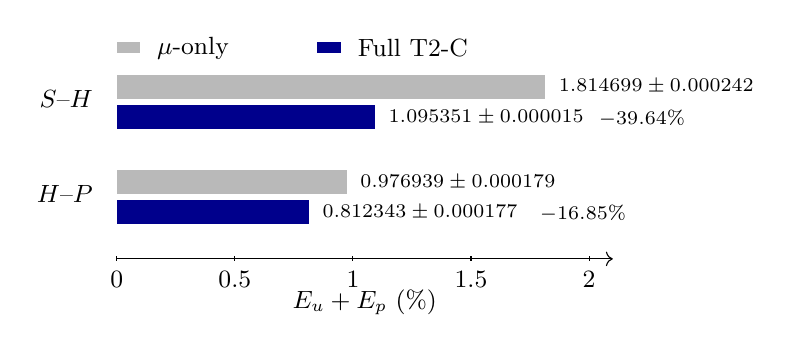
\begin{tikzpicture}[x=3cm,y=0.55cm,font=\small]
\draw[->] (0,0)--(2.1,0);
\node at (1.05,-1.0) {$E_u+E_p$ (\%)};
\foreach \t in {0,0.5,1,1.5,2} {
 \draw (\t,0.06)--(\t,-0.06) node[below] {\t};
}
\node[anchor=east] at (-0.06,3.7) {$S$--$H$};
\node[anchor=east] at (-0.06,1.5) {$H$--$P$};
\fill[gray!55] (0,3.7) rectangle (1.814699,4.25);
\fill[blue!55!black] (0,3.0) rectangle (1.095351,3.55);
\fill[gray!55] (0,1.5) rectangle (0.976939,2.05);
\fill[blue!55!black] (0,0.8) rectangle (0.812343,1.35);
\node[anchor=west,font=\scriptsize] at (1.83,3.975) {$1.814699\pm0.000242$};
\node[anchor=west,font=\scriptsize] at (1.11,3.275) {$1.095351\pm0.000015$};
\node[anchor=west,font=\scriptsize] at (0.99,1.775) {$0.976939\pm0.000179$};
\node[anchor=west,font=\scriptsize] at (0.83,1.075) {$0.812343\pm0.000177$};
\fill[gray!55] (0,4.75) rectangle (0.1,5.0);
\node[anchor=west] at (0.13,4.87) {$\mu$-only};
\fill[blue!55!black] (0.85,4.75) rectangle (0.95,5.0);
\node[anchor=west] at (0.98,4.87) {Full T2-C};
\node[anchor=west,font=\scriptsize] at (2.0,3.25) {$-39.64\%$};
\node[anchor=west,font=\scriptsize] at (1.75,1.05) {$-16.85\%$};
\end{tikzpicture}

\caption{Full-window joint errors at $K=24$ for both centered-square
overlaps. Values are mean $\pm$ sample standard deviation across three
paired gate-training seeds with all candidate trajectories fixed.
The reductions are relative to the architecture-matched $\mu$-only gate.
The field comparisons in Appendix~\ref{app:square} include both
specialists, including the stronger Periodic candidate in $H$--$P$.}
\label{fig:square_overlap}
\end{figure}



The full-window comparison in Figure~\ref{fig:square_overlap} gives the
same direction of effect as the terminal metric: history conditioning
reduces the three-seed mean joint error by $39.64\%$ in $S$--$H$ and
$16.85\%$ in $H$--$P$. These results condition on fixed candidates.
The frozen-checkpoint reevaluation also improves on training-fitted
constant mixing weights and constant-logit offsets
(Appendix~\ref{app:square}).

\subsection{What do matched local controls establish?}

We reevaluate Circular H/P models with common held-out windows and
POD-reconstructed reference fields. The Dense control matches the active
parameter budget of the proposed model; the structured control removes
input-dependent routing. This is distinct from the earlier
Vanilla-FNN-MoE, DataOnly-MoE, and Global MoE comparison, whose summary and
min--max tables are replaced here because their historical aggregation
could not be fully reconciled. The new results do not retroactively
validate those old statistics or isolate every architectural factor.



\begin{table}[H]
\centering
\caption{Circular Periodic controls: full-window mean physical-field
errors (\%) at $K=24$, against POD-reconstructed truth. Entries are mean
$\pm$ sample standard deviation over seeds 1248, 1600, and 2026; all
listed neural configurations have 3/3 accepted seeds. Repaired denotes
the changed quadratic-branch initialization.}
\label{tab:circular_full_reorg}
\small
\setlength{\tabcolsep}{4pt}
\begin{tabular}{@{}lccc@{}}
\toprule
Model & $E_u$ & $E_p$ & $E_u+E_p$\\
\midrule
Proposed, original & $0.5731\pm0.3638$ & $2.3060\pm1.3681$ & $2.8791\pm1.7269$\\
Proposed, repaired & $0.5814\pm0.3949$ & $2.4854\pm1.4427$ & $3.0667\pm1.8373$\\
Dense, active-matched & $\mathbf{0.2446\pm0.0323}$ & $\mathbf{1.0805\pm0.1946}$ & $\mathbf{1.3251\pm0.2268}$\\
Structured, original & $0.5178\pm0.2667$ & $2.3489\pm1.1688$ & $2.8666\pm1.4342$\\
Structured, repaired & $0.5429\pm0.2783$ & $2.3168\pm1.0315$ & $2.8598\pm1.3081$\\
\bottomrule
\end{tabular}
\end{table}



The Dense control is more accurate than both proposed configurations at
$K=24$ and $K=48$ (Appendix~\ref{app:circular}). The routing-free
structured control is close to the proposed model. Thus this study does
not identify sparse local routing as a source of Periodic accuracy under
the matched active-parameter budget.

A checkpoint audit found that the original Circular quadratic branches
remained zero because both multiplicative factors were initialized at
zero. Keeping one factor random activates the branch but does not improve
Periodic accuracy consistently. For Hopf, two of six repaired FP32 runs
still develop non-finite gradients, leaving two accepted seeds per
architecture. We report their errors as accepted-only descriptive
statistics, not complete three-seed estimates.

A regularized polynomial OpInf adaptation is competitive on Hopf
($K=24$ joint error $0.03870\%$) but performs poorly on Periodic
($114.0941\%$). Its pressure map, derivative estimation, and validation
search are documented in Appendix~\ref{app:circular}; these results do
not establish a general advantage over the OpInf method family.

\paragraph{Computational scope.}
Per-decision active parameter counts characterize conditional execution,
not latency. A batch-one native Circular Periodic $K=48$ rollout with
physical decoding takes a median $2.1848$ s for proposed, compared with
$0.6579$ s for Dense. This diagnostic excludes initialization, outer
routing, descriptor construction, and fusion. It therefore provides
neither an end-to-end runtime nor a FOM speedup
(Appendix~\ref{app:parameter_counts}).

\FloatBarrier
\section{Conclusion}
We introduced RAL-MoE-ROM to combine autonomous regime-local predictors
through physical-space assembly while retaining independent reduced
coordinates. On the evaluated centered-square overlaps, physical-history
conditioning improves T2-C over the architecture-matched parameter-only
gate for all three gate-training seeds. The local control experiments
qualify the role of the inner architecture: the active-parameter-matched
Dense control is more accurate on Circular Periodic, and the original
audited quadratic branches remained inactive. Repaired Hopf training
also retains failed seeds. These results support the evaluated local
prediction and output-assembly capabilities, but do not establish sparse
routing or explicit quadratic corrections as necessary sources of
accuracy. The study assumes prescribed regime coverage and supplied
initial physical histories. Full-field CFD errors, nonlinear
constraint preservation, global cross-chart data-role verification,
and end-to-end FOM speedups remain to be established.


\subsubsection*{Reproducibility statement}
The main text reports the benchmark roles, evaluation horizons, baselines, and metrics. Appendices~A--E document the local-coordinate construction, projected operators, specialist architecture, routing and fusion procedure, and implementation details. Appendices~F--H provide benchmark-specific results.
Appendix~\ref{app:internal_routing} reports post-hoc internal-routing statistics
from fixed validation-selected Hopf and Periodic specialists on held-out
rollout windows; these diagnostics are not used for model selection.
Appendix~\ref{app:circular} reports the new Circular control study, initialization audit, and accepted/failed seed counts; Appendix~\ref{app:parameter_counts} separates parameter counts from measured local latency.
Appendix~\ref{app:square} additionally reports an architecture-matched descriptor
ablation and three-seed variability of the centered-square T2-C gate, with the
underlying specialists and E2 router held fixed.

\subsection*{AI use statement}
% Authors must confirm this disclosure against the final submission workflow.
Generative AI tools, including ChatGPT and Codex, assisted with language polishing, LaTeX formatting, consistency checks, experiment-code development, and analysis of experimental records. The authors take full responsibility for reviewing and verifying all scientific
content, mathematical formulations, experimental configurations, numerical
results, and conclusions, and for the final manuscript and all reported results.

\bibliography{references,legacy_references}
\bibliographystyle{iclr2027_conference}

\appendix
\section{Full problem setup and weighted POD construction}
\label{app:problem_pod}

\subsection{Parameterized full-order model, gauge, and regime coverage}

After spatial discretization, the velocity
$\bm u(t;\mu)\in\mathbb R^{N_u}$ and pressure
$p(t;\mu)\in\mathbb R^{N_p}$ satisfy


\begin{equation}
    \dot{\bm u}
    =
    \bm f_h(\mu)
    +\mathcal L_h(\mu)\bm u
    -\mathcal N_h(\bm u,\bm u;\mu)
    -\nabla_h(\mu)p,
    \qquad
    \operatorname{div}_h(\mu)\bm u=0.
    \label{eq:app_fom}
\end{equation}


Pressure is defined only up to an additive constant.
With positive finite-volume weights $\bm w$, each pressure snapshot is mapped
to the weighted zero-mean gauge


\begin{equation}
    \Gamma_p(q)
    =
    q-\frac{\bm w^\top q}{\bm w^\top\bm 1}\bm 1,
    \qquad
    p^\circ=\Gamma_p(p),
    \qquad
    \bm w^\top p^\circ=0.
    \label{eq:app_pressure_gauge}
\end{equation}



The parameter domain is covered by overlapping regime-local parameter regions,


\begin{equation}
    \mathcal M
    \subseteq
    \bigcup_{r\in\{S,H,P\}}\mathcal M_r,
    \qquad
    \mathcal O_{SH}
    =
    \mathcal M_S\cap\mathcal M_H,
    \qquad
    \mathcal O_{HP}
    =
    \mathcal M_H\cap\mathcal M_P,
    \label{eq:app_regime_cover}
\end{equation}


where $S$, $H$, and $P$ denote the steady, Hopf-onset, and periodic
regimes, respectively.
Only adjacent overlaps are used; no direct $S$--$P$ overlap is considered.


\subsection{Area-weighted local POD}

The finite-volume quadrature induces the weighted inner products


\begin{equation}
    \langle\bm v,\bm z\rangle_{M_u}
    =
    \bm v^\top M_u\bm z,
    \qquad
    \langle q,s\rangle_{M_p}
    =
    q^\top M_p s,
    \qquad
    M_p=\operatorname{diag}(\bm w),
    \qquad
    M_u=\operatorname{diag}(M_p,M_p).
    \label{eq:app_weighted_inner_products}
\end{equation}



For chart $r$, let $d_u^{(r)}$ and $d_p^{(r)}$ denote the retained velocity
and pressure dimensions.
Let $X_u^{(r)}$ and $X_p^{(r)}$ collect the centered velocity and
gauge-corrected pressure snapshots from the training trajectories assigned
to that chart.
The corresponding chart-specific means are denoted by
$\bar{\bm u}^{(r)}$ and $\bar p^{(r),\circ}$.
The local POD bases solve


\begin{align}
    \Phi_u^{(r)}
    &\in
    \underset{\Psi^\top M_u\Psi=I_{d_u^{(r)}}}
    {\operatorname{arg\,min}}
    \left\|
        X_u^{(r)}
        -\Psi\Psi^\top M_uX_u^{(r)}
    \right\|_{M_u,F}^2,
    \\
    \Phi_p^{(r)}
    &\in
    \underset{\Psi^\top M_p\Psi=I_{d_p^{(r)}}}
    {\operatorname{arg\,min}}
    \left\|
        X_p^{(r)}
        -\Psi\Psi^\top M_pX_p^{(r)}
    \right\|_{M_p,F}^2,
    \label{eq:app_pod_optimization}
\end{align}


where


\begin{equation}
    \|Y\|_{M,F}^2=\operatorname{tr}(Y^\top MY).
\end{equation}



Equivalently, consider the weighted singular value decompositions


\begin{equation}
    M_u^{1/2}X_u^{(r)}
    =
    U_u^{(r)}\Sigma_u^{(r)}{V_u^{(r)}}^\top,
    \qquad
    M_p^{1/2}X_p^{(r)}
    =
    U_p^{(r)}\Sigma_p^{(r)}{V_p^{(r)}}^\top.
\end{equation}


The retained bases are


\begin{equation}
    \Phi_u^{(r)}
    =
    M_u^{-1/2}
    U_u^{(r)}(:,1{:}d_u^{(r)}),
    \qquad
    \Phi_p^{(r)}
    =
    M_p^{-1/2}
    U_p^{(r)}(:,1{:}d_p^{(r)}),
    \label{eq:app_weighted_svd_bases}
\end{equation}


and satisfy


\begin{equation}
    {\Phi_u^{(r)}}^\top M_u\Phi_u^{(r)}=I,
    \qquad
    {\Phi_p^{(r)}}^\top M_p\Phi_p^{(r)}=I.
\end{equation}


Because the pressure snapshots and their chart mean satisfy the same weighted
gauge condition, the pressure basis also satisfies


\begin{equation}
    \bm w^\top\Phi_p^{(r)}=\bm 0^\top .
\end{equation}



Encoding and decoding are performed independently within each chart:


\begin{align}
    \bm a^{(r)}
    &=
    {\Phi_u^{(r)}}^\top
    M_u
    \bigl(\bm u-\bar{\bm u}^{(r)}\bigr),
    &
    \mathcal D_r^u(\bm a^{(r)})
    &=
    \bar{\bm u}^{(r)}
    +\Phi_u^{(r)}\bm a^{(r)},
    \\
    \bm b^{(r)}
    &=
    {\Phi_p^{(r)}}^\top
    M_p
    \bigl(\Gamma_p(p)-\bar p^{(r),\circ}\bigr),
    &
    \mathcal D_r^p(\bm b^{(r)})
    &=
    \bar p^{(r),\circ}
    +\Phi_p^{(r)}\bm b^{(r)}.
    \label{eq:app_encode_decode}
\end{align}



The reduced coefficients are standardized using chart-local statistics
estimated from the corresponding training trajectories:


\begin{equation}
    \widetilde{\bm a}^{(r)}
    =
    \bigl(
        \bm a^{(r)}-\bm\mu_a^{(r)}
    \bigr)
    \oslash
    \bm\sigma_a^{(r)},
    \qquad
    \widetilde{\bm b}^{(r)}
    =
    \bigl(
        \bm b^{(r)}-\bm\mu_b^{(r)}
    \bigr)
    \oslash
    \bm\sigma_b^{(r)}.
    \label{eq:app_local_scalers}
\end{equation}


Additional specialist features and their normalization are specified in
Appendix~\ref{app:specialists}.

All chart-local means, POD bases, and scaling statistics are constructed
independently.
Consequently, reduced coefficient vectors from different charts are not
assumed to be componentwise comparable; only their decoded physical fields lie in a common physical comparison space.






\section{Projected Galerkin and pressure operators}
\label{app:rom}

\subsection{Chart-local Galerkin momentum dynamics}

For each chart $r\in\{S,H,P\}$, substituting the chart-local affine reconstructions
from Appendix~\ref{app:problem_pod} into the semi-discrete
momentum equation and testing against the local velocity basis yields


\begin{equation}
    \dot{\bm a}^{(r)}
    =
    \bm c_r(\mu)
    +
    A_r(\mu)\bm a^{(r)}
    +
    H_r(\mu):
    \bigl(
        \bm a^{(r)}\otimes\bm a^{(r)}
    \bigr)
    +
    C_r^p(\mu)\bm b^{(r)}.
    \label{eq:app_projected_momentum}
\end{equation}


Here ``$:$'' denotes the double contraction.
For velocity modes
$\bm\phi_i^{u,(r)}$,
$i=1,\ldots,d_u^{(r)}$,
and pressure modes
$\phi_\ell^{p,(r)}$,
$\ell=1,\ldots,d_p^{(r)}$,
the projected operators are


\begin{align}
    [\bm c_r(\mu)]_i
    &=
    \Bigl\langle
        \bm\phi_i^{u,(r)},
        \bm f_h(\mu)
        +
        \mathcal L_h(\mu)\bar{\bm u}^{(r)}
        -
        \mathcal N_h
        \bigl(
            \bar{\bm u}^{(r)},
            \bar{\bm u}^{(r)};
            \mu
        \bigr)
        -
        \nabla_h(\mu)\bar p^{(r),\circ}
    \Bigr\rangle_{M_u},
    \\
    [A_r(\mu)]_{ij}
    &=
    \Bigl\langle
        \bm\phi_i^{u,(r)},
        \mathcal L_h(\mu)\bm\phi_j^{u,(r)}
        -
        \mathcal N_h
        \bigl(
            \bar{\bm u}^{(r)},
            \bm\phi_j^{u,(r)};
            \mu
        \bigr)
        -
        \mathcal N_h
        \bigl(
            \bm\phi_j^{u,(r)},
            \bar{\bm u}^{(r)};
            \mu
        \bigr)
    \Bigr\rangle_{M_u},
    \\
    [H_r(\mu)]_{ijk}
    &=
    -
    \Bigl\langle
        \bm\phi_i^{u,(r)},
        \mathcal N_h
        \bigl(
            \bm\phi_j^{u,(r)},
            \bm\phi_k^{u,(r)};
            \mu
        \bigr)
    \Bigr\rangle_{M_u},
    \\
    [C_r^p(\mu)]_{i\ell}
    &=
    -
    \Bigl\langle
        \bm\phi_i^{u,(r)},
        \nabla_h(\mu)\phi_\ell^{p,(r)}
    \Bigr\rangle_{M_u}.
    \label{eq:app_projected_operators}
\end{align}



We denote the resulting chart-local projected momentum vector field by


\begin{equation}
    \mathcal F_r^G
    \bigl(
        \bm a^{(r)},
        \bm b^{(r)};
        \mu
    \bigr)
    =
    \bm c_r(\mu)
    +
    A_r(\mu)\bm a^{(r)}
    +
    H_r(\mu):
    \bigl(
        \bm a^{(r)}\otimes\bm a^{(r)}
    \bigr)
    +
    C_r^p(\mu)\bm b^{(r)}.
    \label{eq:app_galerkin_backbone}
\end{equation}


This vector field provides the explicit projected Galerkin backbone of the
regime-local specialist introduced in
Eq.~(\plaineqref{eq:main_specialist}).


\subsection{Gauge-consistent pressure--Poisson map}

The pressure component is represented through a chart-local
Pressure--Poisson relation.
At the continuous level, the gauge-corrected pressure satisfies


\begin{equation}
    -\Delta p^\circ
    =
    \nabla\!\cdot
    \left[
        (\bm u\!\cdot\!\nabla)\bm u
        -
        \bm f
    \right],
    \qquad
    \int_\Omega p^\circ\,\mathrm d\Omega=0,
    \label{eq:app_continuous_pressure_poisson}
\end{equation}


with boundary conditions inherited from the momentum equation. The archived Circular Periodic pressure base is a projected weak-form surrogate, not the original finite-volume pressure solve. Its asset metadata explicitly states that boundary terms are neglected.

\paragraph{Verified weak-form construction for Circular Periodic.}
Let $\psi_\ell$ be a pressure mode and $\bm\phi_j$ a velocity mode, and suppress the chart index in the following definitions. The archived construction evaluates gradients using \texttt{pyvista.UnstructuredGrid.compute\_derivative()} on the unstructured source mesh and uses the POD \texttt{point\_areas} as quadrature weights $w_i$. Define


\begin{equation}
 \langle x,y\rangle_w=\sum_i w_i\,x_i\cdot y_i,
 \qquad
 C(v,z)_i=(v_i\cdot G_h)z_i ,
\end{equation}


where $G_h$ denotes this post-processing gradient, not an assertion of equality with the full-order face-flux stencil. With $\bm u=\bar{\bm u}+\sum_j a_j\bm\phi_j$ and $p=\bar p+\sum_m b_m\psi_m$, the saved weak-form system is


\begin{equation}
 K_r^p\bm b^{PP}=\bm d_r+B_r\bm a+Q_r:(\bm a\otimes\bm a),
 \label{eq:app_pressure_poisson_system}
\end{equation}


with


\begin{align}
 [K_r^p]_{\ell m}&=-\langle G_h\psi_\ell,G_h\psi_m\rangle_w,
 \label{eq:app_ppe_K_definition}\\
 [\bm d_r]_\ell&=\langle G_h\psi_\ell,C(\bar{\bm u},\bar{\bm u})+G_h\bar p\rangle_w,
 \label{eq:app_ppe_d_definition}\\
 [B_r]_{\ell j}&=\langle G_h\psi_\ell,C(\bar{\bm u},\bm\phi_j)+C(\bm\phi_j,\bar{\bm u})\rangle_w,
 \label{eq:app_ppe_B_definition}\\
 [Q_r]_{\ell jk}&=\langle G_h\psi_\ell,C(\bm\phi_j,\bm\phi_k)\rangle_w.
 \label{eq:app_ppe_Q_definition}
\end{align}


Here $K_r^p\in\mathbb R^{d_p\times d_p}$, $\bm d_r\in\mathbb R^{d_p}$, $B_r\in\mathbb R^{d_p\times d_u}$, and $Q_r\in\mathbb R^{d_p\times d_u\times d_u}$. The negative sign in $K_r^p$ follows the archived convention $\Delta p=-\nabla\cdot[(\bm u\cdot\nabla)\bm u]$ after integration by parts. The velocity mean generates both constant and linear terms, and the pressure mean contributes to $\bm d_r$. Neglecting the boundary integral is an approximation; it must not be described as incorporation of the exact full-order pressure boundary closure.

The asset stores an SVD pseudoinverse with relative cutoff $10^{-10}$ and the precontracted arrays


\begin{equation}
 \widetilde{\bm c}=(K_r^p)^\dagger\bm d_r,\qquad
 \widetilde A=(K_r^p)^\dagger B_r,\qquad
 \widetilde H=(K_r^p)^\dagger Q_r.
\end{equation}


Online evaluation is therefore


\begin{equation}
 \mathcal Q_r^{PP}(\bm a;\mu)
 =\widetilde{\bm c}(\mu)+\widetilde A(\mu)\bm a+
   \widetilde H:(\bm a\otimes\bm a).
 \label{eq:app_pressure_poisson_map}
\end{equation}


No full-mesh pressure equation is solved online. The Circular Periodic asset has $d_u=d_p=32$, numerical rank 32, and a reported condition estimate of approximately $72.5$. Its metadata and construction report identify a projected polynomial surrogate, rather than a polynomial fitted to pressure targets. This verified provenance is specific to this asset and is not inferred solely from the polynomial form of other archived pressure maps.

A replay of the saved weak-form coefficients at 63 parameter nodes reproduces the online polynomial to a maximum absolute discrepancy of $1.73\times10^{-14}$. This checks algebraic consistency of the stored arrays; it does not reassemble mesh derivatives or validate the original finite-volume residual.

The pressure fields are compared after the common weighted gauge correction. Neither the approximate pressure base, its learned correction, nor the subsequent physical-space fusion is claimed to satisfy the original finite-volume PPE exactly. In particular, a residual evaluated using $G_h$ would be a post-processing consistency diagnostic, not the residual of the original face-flux solver.

The pair


\begin{equation}
    \left(
        \mathcal F_r^G,
        \mathcal Q_r^{PP}
    \right)
\end{equation}


is constructed independently for each regime-local chart.
Accordingly, each chart carries its own parameter region, mean fields,
POD bases, coefficient scalings, projected momentum operators, and
Pressure--Poisson map.
These chart-local operators are used only within their native reduced
coordinates; no componentwise interpolation of reduced states or projected
operators is assumed across charts.


\section{Regime-local specialist architecture and closed-loop training}
\label{app:specialists}

For each regime-local chart $r$, we define a self-contained 
specialist in its native reduced coordinates: velocity is advanced
dynamically, whereas pressure is reconstructed algebraically.
The projected operators from Appendix~\ref{app:rom} provide the underlying physics, while learned terms model unresolved reduced dynamics. The velocity coefficients satisfy


\begin{equation}
  \dot{\bm a}^{(r)}
  =
  \mathcal F_r^G
  \left(
    \bm a^{(r)},\bm b^{(r)};\mu
  \right)
  +
  \bm\rho^u_{\theta_r}
  \left(
    \bm\xi^{(r)}
  \right).
  \label{eq:app_hybrid_velocity_rhs}
\end{equation}


After each reduced velocity time step, pressure is reconstructed through


\begin{align}
  \bm b_{n+1}^{PP,(r)}
  &=
  \mathcal Q_r^{PP}
  \left(
    \bm a_{n+1}^{(r)};\mu
  \right),
  \nonumber\\
  \bm\gamma_n^{(r)}
  &=
  \operatorname{sigmoid}
  \left(
    \bm\eta^p_{\theta_r}
    (\bm\xi_n^{(r)})
  \right),
  \nonumber\\
  \bm b_{n+1}^{(r)}
  &=
  \bm\gamma_n^{(r)}
  \odot
  \bm b_{n+1}^{PP,(r)}
  +
  \bm\rho^p_{\theta_r}
  (\bm\xi_n^{(r)}),
  \qquad
  \bm\gamma_n^{(r)}
  \in(0,1)^{d_p^{(r)}}.
  \label{eq:app_pressure_closure}
\end{align}


The gate modulates the projected Pressure--Poisson contribution, while
$\bm\rho^p_{\theta_r}$ provides the learned pressure correction.


\subsection{Features and structured sparse experts}

Let


\begin{equation}
  \bm g_n^{(r)}
  =
  \mathcal F_r^G
  \left(
    \bm a_n^{(r)},\bm b_n^{(r)};\mu
  \right)
  \label{eq:app_galerkin_feature}
\end{equation}


denote the projected velocity right-hand side defined in Eq.~(\plaineqref{eq:app_galerkin_backbone}). The specialist uses the ordered three-state history


\begin{equation}
  \mathcal H_n^{(r)}
  =
  \left(
    \bm a_{n-\ell}^{(r)},
    \bm b_{n-\ell}^{(r)},
    \bm g_{n-\ell}^{(r)}
  \right)_{\ell=0}^{2},
  \label{eq:app_specialist_history}
\end{equation}


and constructs


\begin{equation}
  \bm\xi_n^{(r)}
  =
  \operatorname{Feat}_r
  \left(
    \mathcal H_n^{(r)},\mu
  \right),
  \qquad
  \bm z_n^{(r)}
  =
  \operatorname{Enc}_r
  \left(
    \bm\xi_n^{(r)}
  \right).
  \label{eq:app_specialist_features}
\end{equation}


The feature map contains standardized local states, projected
right-hand sides and parameter features. All normalization statistics are estimated from the corresponding chart-specific training set. Internal routing first selects an expert group. When group selection is learned,


\begin{equation}
  m^\star
  =
  \underset{m\in\mathcal G_r}{\operatorname{arg\,max}}
  \;
  \pi_{r,m}^{\mathrm{grp}}
  \left(
    \bm z_n^{(r)},\bm\xi_n^{(r)}
  \right),
  \label{eq:app_group_top1}
\end{equation}


whereas $m^\star$ is predetermined for single-group or fixed-group
specialists. Within the selected group, velocity and pressure use separate channel routers. For $c\in\{u,p\}$, let $\mathcal T_2^c$ denote the two routed experts with the largest channel-specific weights. Together with the shared expert $e=0$,


\begin{equation}
  \mathcal M_{\theta_r}^c
  =
  \omega_0^c
  E_{0,m^\star}^c
  +
  \sum_{e\in\mathcal T_2^c}
  \omega_e^c
  E_{e,m^\star}^c,
  \qquad
  \omega_e^c\ge0,
  \qquad
  \omega_0^c+\sum_{e\in\mathcal T_2^c}\omega_e^c=1.
  \label{eq:app_channel_sparse_moe}
\end{equation}


For the audited Circular H/P instances, $\omega_0^c=4/7$ and
$\omega_e^c=(3/7)\,p_e^c/\sum_{j\in\mathcal T_2^c}p_j^c$ for selected
routed experts. This fixed shared/routed split is not assumed for every
benchmark configuration.
The two channel mixtures define the velocity and pressure corrections
$\bm\rho_{\theta_r}^u$ and $\bm\rho_{\theta_r}^p$, respectively. The explicit linear and quadratic branches operate on the channel-specific reduced-state inputs


\begin{equation}
  \bm s^{u,(r)}
  =
  \widetilde{\bm a}^{(r)},
  \qquad
  \bm s^{p,(r)}
  =
  \operatorname{col}
  \left(
    \widetilde{\bm a}^{(r)},
    \widetilde{\bm b}^{(r)}
  \right).
  \label{eq:app_expert_state_slices}
\end{equation}


For output component $j$, each expert is


\begin{align}
  \left[E_{e,m}^c\right]_j
  &=
  \left[
    N_{e,m}^c
    \left(
      \bm z,\bm s^c
    \right)
  \right]_j
  +
  \left[
    W_{e,m}^{c,\mathrm{lin}}
    \bm s^c
  \right]_j
  \nonumber\\
  &\quad+
  \kappa
  \sum_{\ell=1}^{q_b}
  \left(
    {\bm v_{e,m,j\ell}^{c,(1)}}^{\top}
    \bm s^c
  \right)
  \left(
    {\bm v_{e,m,j\ell}^{c,(2)}}^{\top}
    \bm s^c
  \right),
  \qquad
  q_b=4,
  \qquad
  \kappa=0.05.
  \label{eq:app_structured_expert}
\end{align}


Thus each expert combines a nonlinear feature-conditioned response with
explicit linear and low-rank quadratic responses of the local reduced state.


\subsection{Frozen-context advancement and closed-loop training}

During one reduced velocity time step, the current pressure, recent history, and
physical parameter define a context $\mathcal C_n^{(r)}$ that is held fixed
while the velocity state is advanced. We write


\begin{equation}
  F_r
  \left(
    \bm a;\mathcal C_n^{(r)}
  \right)
  =
  \mathcal F_r^G
  \left(
    \bm a,\bm b_n^{(r)};\mu
  \right)
  +
  \bm\rho^u_{\theta_r}
  \left(
    \bm\xi^{(r)}
    \left(
      \bm a;\mathcal C_n^{(r)}
    \right)
  \right).
  \label{eq:app_frozen_context_rhs}
\end{equation}


The chart-specific numerical update is denoted by


\begin{equation}
  \bm a_{n+1}^{(r)}
  =
  \operatorname{Step}_r
  \left(
    \bm a_n^{(r)};
    F_r(\cdot;\mathcal C_n^{(r)}),
    \Delta t_r
  \right).
  \label{eq:app_specialist_step}
\end{equation}


Continuous-time specialist instances use Runge--Kutta integration with the
same frozen context across stage evaluations; benchmark-specific stepping
details are reported in Appendix~\ref{app:implementation}.
The nominal Runge--Kutta order applies to this frozen-context velocity subproblem, not automatically to the complete pressure/history-coupled update. We do not claim fourth-order convergence of the full scheme.
The updated velocity is then supplied to
Eq.~(\plaineqref{eq:app_pressure_closure}), after which the history is
shifted and autonomous rollout continues.

For a closed-loop rollout of length $K$, the specialist recursively
consumes its own predicted states and minimizes


\begin{equation}
  \mathcal L_r
  =
  \frac{1}{K}
  \sum_{k=1}^{K}
  \left[
    \frac{1}{d_u^{(r)}}
    \left\|
      \left(
        \widehat{\bm a}_{n+k}^{(r)}
        -
        \bm a_{n+k}^{(r)}
      \right)
      \oslash
      \bm\sigma_a^{(r)}
    \right\|_2^2
    +
    \frac{1}{d_p^{(r)}}
    \left\|
      \left(
        \widehat{\bm b}_{n+k}^{(r)}
        -
        \bm b_{n+k}^{(r)}
      \right)
      \oslash
      \bm\sigma_b^{(r)}
    \right\|_2^2
  \right].
  \label{eq:app_true_rollout_loss}
\end{equation}


After initialization, no reference state inside the prediction window is
injected into the autonomous rollout. Training uses progressively longer
chart-specific rollout horizons; the corresponding curricula and
optimization settings are listed in Appendix~\ref{app:implementation}.


\paragraph{Initialization audit.}
In the audited original Circular checkpoints, both factors of the
multiplicative quadratic branch were initialized at zero and remained
zero, since the gradient of either factor contains the other factor.
The repaired configuration retains a random right factor and zeroes only
the left factor, preserving zero initial output with a nonzero learning
direction. The repair activates this branch but does not establish an
accuracy benefit; see Appendix~\ref{app:circular}.

\paragraph{Loss interpretation.}
Variance normalization weights coefficient errors by inverse training
variance and is distinct from the physical energy norm. The equality
$\|\Phi(\widehat a-a)\|_M^2=\|\widehat a-a\|_2^2$ holds within a common
weighted-orthonormal chart; comparison to original CFD fields additionally
involves the projection remainder. Neither loss alone guarantees
conservation or long-term stability.

\section{Outer routing and T2-C details}
\label{app:routing}

\paragraph{Parameter-only regime routing.}
The E2 router receives only the standardized scalar parameter,


\begin{equation}
  \widetilde\mu
  =
  \frac{\mu-\mu_R}{\sigma_R},
  \qquad
  \bm\pi(\mu)
  =
  \operatorname{softmax}
  \left(
    \mathcal R_{E2}(\widetilde\mu)
  \right)
  =
  [\pi_S,\pi_H,\pi_P]^\top .
  \label{eq:app_e2_parameter_only}
\end{equation}


The trajectory-level preference is evaluated once and remains fixed
throughout the subsequent rollout. The regime graph contains only adjacent transitions,


\begin{equation}
  \mathcal E_{\rm adj}
  =
  \bigl\{
    \{S,H\},
    \{H,P\}
  \bigr\},
  \label{eq:app_adjacency}
\end{equation}


so direct $S$--$P$ fusion is excluded.
Let
$m_j(\mathcal H_n,\mu,K)\in\{0,1\}$
denote the validation-supported applicability of specialist $j$ for the
given initialization and rollout horizon.
The regularized E2 weight restricted to applicable specialists is


\begin{equation}
  \widetilde\pi_j
  =
  \frac{
    m_j\pi_j
  }{
    \sum_{k\in\{S,H,P\}}m_k\pi_k+\varepsilon
  }.
  \label{eq:app_masked_e2}
\end{equation}


For $Z=\sum_k m_k\pi_k>0$, these regularized weights sum to $Z/(Z+\varepsilon)$, rather than exactly one. They preserve the ranking of applicable specialists; the selected pair is normalized separately below. A single applicable specialist yields the Top-1 prediction.
Top-2 fusion is considered only for an applicable pair belonging to
$\mathcal E_{\rm adj}$.
If no specialist is applicable, the hierarchy abstains from prediction. This is the general interface contract, not an experimentally validated out-of-distribution detector. In the reported centered-square overlap implementation, the evaluation cache specifies a fixed candidate pair, $(S,H)$ or $(P,H)$, and $K=24$. E2 Top-1 chooses within this supplied pair and T2-C blends its two independently generated trajectories. These experiments evaluate conditional routing and assembly on prescribed overlap support; they do not test a learned history-dependent mask, the three-applicable case, or abstention coverage on arbitrary new inputs.

We use the canonical ordered pairs $(r_1,r_2)=(S,H)$ and $(P,H)$, including in all tables reporting candidate weights. Reversing the order replaces $\alpha$ by $1-\alpha$ and reverses the corresponding logit sign. For an ordered selected pair $(r_1,r_2)$, the pair-normalized E2
preference is


\begin{equation}
  \bar\pi_1
  =
  \frac{\pi_{r_1}}
       {\pi_{r_1}+\pi_{r_2}},
  \qquad
  \bar\pi_2
  =
  1-\bar\pi_1,
  \qquad
  \ell^{E2}
  =
  \log
  \frac{\bar\pi_1+\varepsilon}
       {\bar\pi_2+\varepsilon}.
  \label{eq:app_pair_logit}
\end{equation}




\paragraph{Chart-independent physical-history descriptor.}
The centered-square implementation uses eight descriptor channels and one parameter input. These features are computed from the initial three physical states at $t_{n-2}<t_{n-1}<t_n$, with pressure mapped to the common zero-mean gauge. They are independent of the specialists' POD coordinates. All quantities below use the nondimensional data conventions of the experiment, and $\epsilon=10^{-12}$ is the numerical floor.

Define $A_\Omega=\sum_i w_i$, $U_j=\|\bm u_j\|_{M_u}^2$, $P_j=\|p_j^\circ\|_{M_p}^2$, and


\begin{align}
 h_j&=\max(t_j-t_{j-1},\epsilon),&
 s_j^u&=\sqrt{\max(U_j,\epsilon)},&
 s_j^p&=\sqrt{\max(P_j,\epsilon)},\\
 v_j&=(\bm u_j-\bm u_{j-1})/h_j,&
 g_j&=\frac{\log\max(U_j,\epsilon)-\log\max(U_{j-1},\epsilon)}{h_j}.
\end{align}


The ordered raw descriptor is


\begin{equation}
\bm s_n=\operatorname{col}\left(
\begin{array}{l}
 \tfrac12\log\max(U_n/A_\Omega,\epsilon),\\
 \tfrac12\log\max(P_n/A_\Omega,\epsilon),\\
 \log(1+\|v_n\|_{M_u}/(s_n^u+\epsilon)),\\
 \log(1+\|v_{n-1}\|_{M_u}/(s_{n-1}^u+\epsilon)),\\
 \tanh(g_n),\\
 \tanh(g_n-g_{n-1}),\\
 \log(1+\|p_n^\circ-p_{n-1}^\circ\|_{M_p}/[h_n(s_n^p+\epsilon)]),\\
 \log(1+\|v_n-v_{n-1}\|_{M_u}/(s_n^u+\epsilon))
\end{array}\right).
\label{eq:app_t2c_descriptor}
\end{equation}


The last channel measures a difference of velocity rates: it is not divided again by a time interval and is not the second-derivative descriptor in an acceleration discretization. The log and hyperbolic-tangent transformations above are part of the actual feature construction.

For the gate, the nine raw features $[\mu;\bm s_n]$ are standardized using the means and population standard deviations of training windows only. Any feature standard deviation below $10^{-8}$ is replaced by one. We denote the resulting vector by $[\widetilde\mu;\bm d_n]$; its parameter normalization is fitted for the gate and need not equal the trajectory-level E2 normalization. The architecture-matched $\mu$-only control sets all eight descriptor channels to zero after standardization. No state from inside the prediction window is used to construct these features.


\paragraph{Physical-space T2-C fusion.}
The logit-correction network receives
$[\widetilde\mu;\bm d_n]\in\mathbb R^9$ and uses two hidden layers of width 64 with SiLU
activations followed by a scalar linear output (9--64--64--1; 4,865 trainable parameters).
The final layer is initialized at zero, so the initial correction vanishes
and the fusion weight reduces to the E2 pair preference.
Specifically,


\begin{equation}
  \Delta_\psi
  =
  c_\psi
  \left(
    [\widetilde\mu;\bm d_n]
  \right),
  \qquad
  \alpha
  =
  \operatorname{sigmoid}
  \left(
    \ell^{E2}+\Delta_\psi
  \right).
  \label{eq:app_t2c_gate}
\end{equation}



The two selected specialists encode the same physical history in their
respective local charts and then evolve independently.
The scalar $\alpha$ is fixed throughout the prediction window and is shared
by velocity and pressure.
After reconstruction on the common physical mesh, T2-C forms


\begin{equation}
  \widehat{\bm q}_{\alpha}^{\,c}(t)
  =
  \alpha\,
  \widehat{\bm q}_{1}^{\,c}(t)
  +
  (1-\alpha)\,
  \widehat{\bm q}_{2}^{\,c}(t),
  \qquad
  c\in\{u,p\},
  \label{eq:app_t2c_field_fusion}
\end{equation}


where the pressure field is gauge corrected.
The fused field is an output only and is never projected back into either
specialist.

The correction network is trained directly on the reconstructed physical
fields. For rollout windows $w$ and prediction steps $k$,


\begin{equation}
  \mathcal L_{\rm T2C}
  =
  \operatorname{mean}_{w,k}
  \left[
    \frac{
      \left\|
        \widehat{\bm u}_{\alpha}^{(w,k)}
        -
        \bm u_{\rm true}^{(w,k)}
      \right\|_{M_u}^2
    }{
      \left\|
        \bm u_{\rm true}^{(w,k)}
      \right\|_{M_u}^2+\varepsilon
    }
    +
    \frac{
      \left\|
        \widehat p_{\alpha}^{\circ,(w,k)}
        -
        p_{\rm true}^{\circ,(w,k)}
      \right\|_{M_p}^2
    }{
      \left\|
        p_{\rm true}^{\circ,(w,k)}
      \right\|_{M_p}^2+\varepsilon
    }
  \right].
  \label{eq:app_t2c_loss}
\end{equation}


Optimization and checkpoint-selection details are reported in
Appendix~\ref{app:implementation}.

\paragraph{Numerical convention in the centered-square evaluator.}
The archived implementation normalizes the selected E2 probabilities, clips the first probability to $[10^{-6},1-10^{-6}]$, and then forms its logit. Its squared relative field loss uses $\max(\|q_{\rm true}\|_M^2,10^{-12})$ as denominator rather than an additive regularizer. Feature standard deviations below $10^{-8}$ are replaced by one before standardization. These are implementation-specific safeguards; the generic additive-$\varepsilon$ notation above should not be read as a claim that all numerical constants or normalization rules are shared across benchmarks.

\section{Reproducibility and implementation details}
\label{app:implementation}

\paragraph{Physical-field error metrics.}
We evaluate reconstructed velocity and gauge-corrected pressure using the relative weighted field errors


\begin{equation}
E_u(n)
=
100\frac{
\|\widehat{\bm u}_n-\bm u_n\|_{M_u}
}{
\|\bm u_n\|_{M_u}
},
\qquad
E_p(n)
=
100\frac{
\|\widehat p_n^\circ-p_n^\circ\|_{M_p}
}{
\|p_n^\circ\|_{M_p}
}.
\label{eq:field_errors}
\end{equation}


Here $\|\bm v\|_M=(\bm v^\top M\bm v)^{1/2}$ uses the finite-volume
quadrature introduced in Appendix~\ref{app:problem_pod}; the velocity norm includes both components, and $p^\circ$ denotes pressure in the common zero-mean gauge. Unless stated otherwise, benchmark-specific temporal and trajectory aggregation is reported with the corresponding experiment. Whenever a joint score is reported,
$E_{\mathrm{joint}}=E_u+E_p$. Independently rounded component values may therefore differ slightly from the displayed joint score.


\paragraph{Trajectory-level partitioning.}
Table~\ref{tab:chart_splits} summarizes the resulting chart-wise parameter coverage, reduced dimensions, trajectory splits, and evaluation horizons. All splits are defined at the level of complete parameter trajectories rather than individual snapshots or rollout windows. Local bases, normalization statistics, and model parameters are constructed from training trajectories only; validation trajectories are used for model and checkpoint selection, and test trajectories are reserved for the reported evaluations. 

\par


\begin{table}[H]
\centering
\caption{
Chart-wise parameter coverage, reduced dimensions, trajectory splits, and evaluation horizons. Counts refer to complete parameter trajectories, and $K$ denotes the number of autonomous rollout steps used for the corresponding local evaluation.
}
\label{tab:chart_splits}
\small
\setlength{\tabcolsep}{3.5pt}
\begin{tabular}{@{}llrrrrrr@{}}
\toprule
Benchmark & Chart & $Re$ range & $(r_u,r_p)$ & Train & Val. & Test & $K$ \\
\midrule
Circular cylinder
& $S$ & 20.0--46.4 & $(32,32)$ & 14 & 2 & 4 & 56 \\
& $H$ & 45.5--59.2 & $(32,32)$ & 29 & 2 & 3 & 56 \\
& $P$ & 57.3--200 & $(32,32)$ & 53 & 6 & 4 & 48 \\
\addlinespace
Centered square
& $S$ & 50--95.4 & $(5,4)$ & 60 & 5 & 4 & 16 \\
& $H$ & 94--102 & $(11,11)$ & 23 & 6 & 5 & 48 \\
& $P$ & 98.5--150 & $(28,26)$ & 27 & 6 & 4 & 24 \\
\addlinespace
Fluidic pinball
& $S$ & 10--19 & $(4,3)$ & 37 & 8 & 7 & 56 \\
& $H$ & 16.6--25 & $(5,5)$ & 39 & 8 & 7 & 56 \\
& $P$ & 21.25--60 & $(17,16)$ & 47 & 9 & 9 & 32 \\
\bottomrule
\end{tabular}
\end{table}


\par


\paragraph{Centered-square T2-C gate optimization.}
Both full T2-C and the architecture-matched $\mu$-only gate use AdamW
(learning rate $3\times10^{-4}$, weight decay $10^{-4}$), 8,000 steps,
and gradient-norm clipping at 1. Minibatches sample training windows with
replacement. Validation is evaluated at step 1 and every 100 steps;
checkpoint selection minimizes the largest Reynolds-number-wise full-window mean joint
error, breaking ties by the pooled mean, without test-based selection.
The paired-seed evaluation is reported in Appendix~\ref{app:square}.



\paragraph{Autonomous rollout protocol.}
All reported specialist evaluations are autonomous after initialization from the prescribed physical history: no reference state from inside the prediction window is injected during rollout.
Each specialist is advanced using its chart-specific time-advancement rule described in Appendix~\ref{app:specialists}. For continuous-time instances, Runge--Kutta stage evaluations share the same frozen pressure/history context within one reduced velocity time step. After each reduced time step, the pressure reconstruction and local history are updated before the next autonomous prediction.


\paragraph{Benchmark discretization and sampling.}
The centered-square dataset contains 120 complete trajectories over
$Re\in[50,150]$ on a 9,400-cell finite-volume mesh. The CFD time step is $\delta t_{\rm CFD}=0.02$, and snapshots are stored every 200 CFD steps, giving $\Delta t_{\rm snap}=4$. The fluidic-pinball dataset contains 131 complete trajectories over $Re\in[10,60]$ on a 70,194-cell mesh, with $\delta t_{\rm CFD}=0.005$ and a snapshot interval of $0.25$ physical time units. The circular-cylinder dataset contains 100 Reynolds-parameterized trajectories spanning
$Re\in[20,200]$ on a common finite-volume mesh represented by 97,368 spatial points. Trajectories contain different numbers of snapshots, yielding 14,167 snapshots in total. The unsteady simulations employ adaptive CFD time stepping subject to $Co_{\max}=0.8$ and $\delta t_{\max}=0.2$, while the snapshot interval is adjusted according to the estimated vortex-shedding period, with eight snapshots retained per shedding cycle. The chart-wise parameter ranges, reduced dimensions, splits, and evaluation horizons are summarized in Table~\ref{tab:chart_splits}.


\paragraph{Specialist optimization.}
Table~\ref{tab:specialist_training} summarizes the reported training configurations, which use AdamW with chart-specific learning rates, weight decay, and rollout curricula.
Additional batching, scheduler, and precision settings are provided in the supplementary implementation.

\par


\begin{table}[H]
\centering
\caption{
Reported specialist training configurations. ``Selected'' denotes the validation-selected checkpoint. The curriculum and budget describe the configured schedule, which may extend beyond the selected checkpoint.
}
\label{tab:specialist_training}
\small
\setlength{\tabcolsep}{3.5pt}
\begin{tabular}{@{}lccccc@{}}
\toprule
Specialist & Initial lr & Weight decay & Rollout curriculum & Budget & Selected \\
\midrule
Circular $S$
& $1.55{\times}10^{-5}$ & $1.0{\times}10^{-4}$
& 4,8,16 & 3600 steps & 1200 steps \\
Circular $H$
& $1.0{\times}10^{-3}$ & $1.0{\times}10^{-4}$
& 1,2,4,8 & 8000 steps & 7200 steps \\
Circular $P$
& $5.5{\times}10^{-4}$ & $1.5{\times}10^{-4}$
& 4,8,12,16 & 240 epochs & 85 epochs \\
\addlinespace
Square $S$
& $1.55{\times}10^{-5}$ & $1.0{\times}10^{-4}$
& 1,4,8,16 & 4000 steps & 3200 steps \\
Square $H$
& $1.0{\times}10^{-3}$ & $1.0{\times}10^{-4}$
& 1,2,4,8 & 8000 steps & 7200 steps \\
Square $P$
& $5.5{\times}10^{-4}$ & $1.5{\times}10^{-4}$
& 4,8,12,16 & 720 epochs & 490 epochs \\
\addlinespace
Pinball $S$
& $1.0{\times}10^{-3}$ & $1.0{\times}10^{-4}$
& 4,8,16 & 8000 steps & 400 steps \\
Pinball $H$
& $1.0{\times}10^{-3}$ & $1.0{\times}10^{-4}$
& 4,8,16,32,56 & 8000 steps & 8000 steps \\
Pinball $P$
& $1.0{\times}10^{-3}$ & $1.0{\times}10^{-4}$
& 4,8,16,24,32 & 8000 steps & 8000 steps \\
\bottomrule
\end{tabular}
\end{table}


\par

\paragraph{Distinct gate objectives.}
Gate fitting minimizes the full-window squared relative field loss in Eq.~(\plaineqref{eq:app_t2c_loss}). Validation selection instead uses the worst-parameter full-window mean of $E_u+E_p$, with the pooled mean as a tie-breaker. The centered-square main comparison reports terminal-step errors; Table~\ref{tab:t2c_window_seeds} additionally reports full-window means. These objectives differ in temporal aggregation, squaring, and parameter weighting. An oracle optimized for a full-window objective is an a posteriori diagnostic, not a guaranteed lower bound for terminal-step error. Three gate-training seeds quantify conditional gate variability, not full-pipeline uncertainty or a confidence interval over independent trajectories.

\paragraph{Verified centered-square E2 configuration.}
The parameter-only router is an MLP $1\to24\to3$ with a Tanh hidden activation and 123 trainable parameters. The scalar Reynolds number is standardized using training-trajectory mean and population standard deviation; a standard deviation below $10^{-7}$ is replaced by one. Each chart-assigned trajectory supplies its chart label. A parameter occurring in more than one chart can therefore produce multiple labeled rows, rather than an assumed unique bifurcation label. The loss is class-weighted cross entropy plus $0.05\,\operatorname{mean}(\pi_S\pi_P)$, with class weight $N/(3N_c)$. Training uses AdamW (learning rate $3\times10^{-4}$, weight decay $10^{-4}$), a cosine schedule over 8,000 steps ending at $1.5\times10^{-5}$, sampling with replacement in batches of $\min(256,N)$, and gradient-norm clipping at one. Selection maximizes validation balanced accuracy plus macro-F1 minus $10^{-3}$ times the current training-batch loss, rather than validation cross entropy alone. For the archived centered-square run, seed 20260730 selects step 3300. These settings describe that verified router, not an assumed common configuration for all benchmarks.

\paragraph{Scope of the hybrid formulation.}
The archived centered-square overlap evaluator loads a Hopf checkpoint through a data-only advancement path: the Galerkin right-hand side enters its features, but is not added to the learned velocity output, and pressure is a learned algebraic output. Consequently, the overlap study tests assembly of frozen local predictors and should not be interpreted as verifying the additive hybrid formulation for every candidate. This implementation distinction does not change the reported overlap numbers or the output-only fusion protocol.

\paragraph{Audited circular-cylinder architectures.}
For the two specialists used in the internal-routing analysis, the Hopf model has input width 493, encoder width 256, one fixed group, and four expert residual blocks with expansion width 1024; the Periodic model has input width 501, encoder width 224, three groups, and three expert residual blocks with expansion width 768. Each group has six routed experts and one shared expert per channel. The encoder has three linear layers with LayerNorm and SiLU, followed by two refinement residual blocks; dropout is 0.04. These configurations identify the analyzed models and are not a substitute for a verified nine-specialist and baseline configuration manifest.

\paragraph{Reference fields and reporting scope.}
The new circular-cylinder control study and centered-square cache-based
reevaluation use POD-reconstructed reference fields. Their errors measure
prediction error in physical space relative to these reconstructions and
do not include the POD projection remainder relative to the original CFD
fields. The original CFD total error and the POD projection error require
a separate aligned-field evaluation. The nominal chart-wise splits above
do not by themselves establish a global cross-chart data-role audit.

\paragraph{Training and evaluation lengths.}
The configured maximum rollout lengths in Table~\ref{tab:specialist_training}
are $16,8,16$ for both Circular and Square $S,H,P$, and $16,56,32$ for
Pinball $S,H,P$. These are training budgets, not the local evaluation
horizons in Table~\ref{tab:chart_splits}. The new Circular H/P comparison
uses $K=24,48$, while Square overlaps use $K=24$. The selected checkpoint
may precede the end of its configured curriculum.

\section{Circular-cylinder controlled reevaluation}
\label{app:circular}

\paragraph{Common evaluation protocol.}
The new study uses seeds 1248, 1600, and 2026. Hopf has 42 windows
from $Re=47.081355,49.022357,51.786450$; Periodic has 32 windows from
$Re=70.314635,100.352251,149.059229,189.862278$. Each window contains
48 prediction steps; $K=24$ uses its first 24 steps. We average relative
physical-field errors over steps, then windows within each Reynolds
number, then equally over Reynolds numbers. Means and sample standard
deviations are computed over the accepted seeds. All reference fields
are reconstructed from true POD coefficients on the corresponding basis.
Only checkpoints accepted by the original validation rule are evaluated
on held-out windows. The training configurations in
Table~\ref{tab:specialist_training} describe the archived original
specialists, not the selected checkpoints of these repeated runs.

\paragraph{Controls and scope.}
Dense matches the active parameter budget, rather than total stored
parameters or execution time. Structured retains explicit response
branches but removes input-dependent expert routing. Neither control
is identical to the older Vanilla-FNN-MoE or Global MoE configuration.
The former Circular summary and min--max tables are replaced by this
explicitly aggregated evaluation. No claim about the former Steady
architecture comparison is inferred from the present H/P results.



\begin{table}[H]
\centering
\caption{Circular Periodic full-window errors (\%) at $K=48$ against
POD-reconstructed truth. All neural rows have 3/3 accepted seeds.
OpInf is one deterministic validation-selected fit.}
\label{tab:circular_full}
\small
\setlength{\tabcolsep}{3pt}
\begin{tabular}{@{}lccc@{}}
\toprule
Model & $E_u$ & $E_p$ & $E_u+E_p$\\
\midrule
Proposed, original & $1.0107\pm0.6513$ & $3.9337\pm2.5070$ & $4.9443\pm3.1576$\\
Proposed, repaired & $1.1040\pm0.7840$ & $4.4282\pm2.8786$ & $5.5322\pm3.6623$\\
Dense, active-matched & $\mathbf{0.4790\pm0.1208}$ & $\mathbf{1.9208\pm0.5391}$ & $\mathbf{2.3998\pm0.6599}$\\
Structured, original & $1.0405\pm0.5015$ & $4.2406\pm2.0664$ & $5.2810\pm2.5679$\\
Structured, repaired & $0.9983\pm0.4944$ & $4.0693\pm1.8827$ & $5.0677\pm2.3762$\\
OpInf & 17.6639 & 97.3258 & 114.9897\\
\bottomrule
\end{tabular}
\end{table}



\paragraph{Quadratic-branch audit.}
The two accepted original Hopf proposed checkpoints each contain 28
quadratic-factor tensors, all zero. The three original Periodic
proposed checkpoints each contain 84 such tensors, all zero; the three
Periodic structured checkpoints each contain four, also all zero.
Thus the original results cannot establish a contribution from the
explicit quadratic branch. The repaired initialization keeps one factor
random and the other zero. Smoke training updates all 14 factor pairs
for Hopf proposed, 42 for Periodic proposed, and two for Periodic
structured. This verifies learning activity, not improved generalization.
For Periodic proposed, the mean joint error increases by $6.52\%$ at
$K=24$ and $11.89\%$ at $K=48$ after repair. Retraining changes the
optimization trajectory and checkpoint selection, so the difference is
not a pure isolated estimate of the quadratic term's effect.



\begin{table}[H]
\centering
\caption{Hopf training completion and validation acceptance.
Counts are over three attempted seeds per architecture; failed runs
are not silently omitted from the denominator.}
\label{tab:hopf_completion}
\small
\begin{tabular}{@{}lccp{5.8cm}@{}}
\toprule
Configuration & Proposed & Structured & Failure or rejection\\
\midrule
Original & 2/3 & 3/3 & Proposed seed 1600 not accepted by validation\\
Repaired, AMP & 0/3 & 0/3 & Non-finite gradients\\
Repaired, FP32 & 2/3 & 2/3 & Proposed 2026: step 3220; structured 1248:
step 2860, both during $K=4$\\
\bottomrule
\end{tabular}
\end{table}





\begin{table}[H]
\centering
\caption{Hopf accepted-only joint errors (\%) against POD-reconstructed
truth, using the common full-window metric. Error bars are sample
standard deviations over accepted seeds only. Rows with 2/3 are
descriptive and are not complete three-seed estimates.}
\label{tab:hopf_accepted}
\small
\begin{tabular}{@{}lccc@{}}
\toprule
Model & $K=24$ & $K=48$ & Accepted\\
\midrule
Proposed, original & $0.11521\pm0.08694$ & $0.11487\pm0.10033$ & 2/3\\
Dense, active-matched & $0.15406\pm0.16364$ & $0.15480\pm0.15525$ & 2/3\\
Proposed, repaired FP32 & $0.04334\pm0.02379$ & $0.05044\pm0.03439$ & 2/3\\
Structured, original & $0.12537\pm0.04614$ & $0.12724\pm0.04302$ & 3/3\\
Structured, repaired FP32 & $0.02229\pm0.00432$ & $0.02392\pm0.00778$ & 2/3\\
OpInf & 0.03870 & 0.05340 & Deterministic\\
\bottomrule
\end{tabular}
\end{table}



The original Dense control also has only two accepted seeds out of three.
The accepted seed sets differ between original and repaired runs.
Consequently, their lower accepted-only errors do not establish improved
expected three-seed performance. FP32 passes the initial 116-combination
preflight (29 training parameters and four curriculum lengths), but this
does not guarantee finite gradients later in optimization.
\DIFaddbegin \DIFadd{For the repaired FP32 runs, the observed training-failure rate is therefore
$1/3$ for each architecture ($2/6$ pooled across these two configurations).
The earlier repaired AMP campaign failed for all six attempted runs;
it is a separate configuration and is not pooled with FP32 to estimate
the latter's failure rate. Validation rejection in the original campaign
is also distinct from a non-finite-gradient training failure. We make no
complete three-seed Hopf robustness claim and do not replace failed seeds
with post-hoc retries in the reported means.
}\DIFaddend 

\paragraph{OpInf adaptation.}
The regularized polynomial model uses constant, linear, compact quadratic,
standardized $1/Re$, and parameter--state interaction features.
Training-trajectory derivatives are estimated by second-order numerical
differentiation. Ridge regularization is selected on validation windows;
a non-finite window invalidates a candidate. Prediction uses fixed RK4
with four substeps per output interval. Pressure is an algebraic ridge
output using the same polynomial features, rather than the proposed
PPE-plus-correction map. Test windows, reference reconstructions, and
quadrature agree with the neural comparison. This is a task-specific
OpInf adaptation, not a reproduction of every detail of an external
implementation.

At $K=24$, OpInf gives $(E_u,E_p,E_{\mathrm{joint}})=
(0.00585,0.03285,0.03870)\%$ on Hopf and
$(15.8676,98.2264,114.0941)\%$ on Periodic.
The Periodic ridge choice lies at the upper boundary of the searched
grid (100), which limits interpretation of that failure. The Hopf result
shows that the method is competitive in the near-onset regime; the
Periodic result does not justify a general claim against OpInf.

\FloatBarrier

\section{Centered-square results}
\label{app:square}


This appendix provides the complete centered-square overlap results
underlying the main-text routing and fusion comparison. Table~\ref{tab:square_fusion_full} reports the velocity, pressure,
and joint errors for the individual specialists and the fusion baselines in the $S$--$H$ and $H$--$P$ overlap regions. In the main text, ``Best fixed'' denotes the fixed specialist with the
lowest aggregate joint error over the corresponding overlap, whereas the convex oracle is a window-wise a posteriori reference.



\paragraph{Overlap evaluation and descriptor ablation.}
For both overlaps, $E_u$, $E_p$, and $E_{\mathrm{joint}}=E_u+E_p$ are reported at the terminal rollout step ($k=24$) and averaged over 16 held-out windows.  This terminal metric differs from the full-window objective used by the diagnostic convex oracle. To assess the role of history information in the second routing level, we also include T2-C $\mu$-only, which uses the same correction-gate architecture and training protocol as T2-C but removes the standardized history descriptor by setting its channels to zero. Table~\ref{tab:square_fusion_full} reports the validation-selected comparison, and the corresponding three-seed gate variability is summarized separately below.

\par


\begin{table}[H]
\centering
\caption{
Centered-square routing and fusion errors at $K=24$. The convex oracle is an a posteriori reference unavailable during prediction.
T2-C $\mu$-only uses the same gate architecture as T2-C but removes the standardized history descriptor. Bold indicates the best deployable method within each overlap.
}
\label{tab:square_fusion_full}
\small
\setlength{\tabcolsep}{5pt}
\begin{tabular}{@{}llrrr@{}}
\toprule
Overlap & Predictor & $E_u$ & $E_p$ & $E_{\mathrm{joint}}$ \\
\midrule
$S$--$H$ & Steady specialist & 2.5976 & 2.2450 & 4.8426 \\
 & Hopf specialist & 0.4942 & 1.2356 & 1.7298 \\
 & E2 Top-1 & 0.4942 & 1.2356 & 1.7298 \\
 & Equal blend & 1.3644 & 1.6677 & 3.0321 \\
 & E2-probability blend & 0.7898 & 1.3949 & 2.1847 \\
 & T2-C $\mu$-only & 0.7898 & 1.3948 & 2.1846 \\
 & T2-C & \textbf{0.4615} & \textbf{0.7343} & \textbf{1.1958} \\
 & Convex oracle & 0.4659 & 0.7183 & 1.1842 \\
\midrule
$H$--$P$ & Periodic specialist & 0.6420 & 0.5659 & 1.2079 \\
 & Hopf specialist & 1.0034 & 1.8684 & 2.8718 \\
 & E2 Top-1 & 0.7422 & 1.1052 & 1.8473 \\
 & Equal blend & 0.6077 & 1.0069 & 1.6146 \\
 & E2-probability blend & 0.6154 & 1.0464 & 1.6618 \\
 & T2-C $\mu$-only & 0.5875 & 0.5629 & 1.1504 \\
 & T2-C & \textbf{0.4509} & \textbf{0.3956} & \textbf{0.8465} \\
 & Convex oracle & 0.4479 & 0.3905 & 0.8384 \\
\bottomrule
\end{tabular}
\end{table}


\par

\par


\begin{table}[H]
\centering
\caption{
Parameter-wise centered-square routing and T2-C results at $K=24$.
Joint errors and relative reductions are reported in percent.
The mean weight is the Steady-specialist weight for $S$--$H$
and the Periodic-specialist weight for $H$--$P$.
}
\label{tab:square_parameter}
\small
\setlength{\tabcolsep}{3.5pt}
\begin{tabular}{lrlrrrr}
\toprule
Overlap & $Re$ & E2 choice & $\bar\alpha$ & E2 $E_{\mathrm{joint}}$ & T2-C $E_{\mathrm{joint}}$ & Reduction \\
\midrule
$S$--$H$ & 95.1 & Hopf & 0.0967 & 1.7140 & 1.1827 & 31.00\% \\
$S$--$H$ & 95.3 & Hopf & 0.0971 & 1.7456 & 1.2090 & 30.74\% \\
$H$--$P$ & 100.5 & Hopf & 0.5870 & 2.6485 & 0.8571 & 67.64\% \\
$H$--$P$ & 102.0 & Periodic & 0.7094 & 1.0462 & 0.8360 & 20.09\% \\
\bottomrule
\end{tabular}
\end{table}


\par

The regime-local specialists also exhibit low aggregate physical-field errors under their respective held-out evaluations: $(E_u,E_p)=(1.5311,1.4583)\%$ in the Steady regime, $(0.4387,0.4844)\%$ in the Hopf regime, and $(0.9395,1.0921)\%$ in the Periodic regime. Within the overlap evaluations, however, the more accurate individual specialist differs by interface: the Hopf specialist is the better single-model reference in $S$--$H$, whereas the Periodic specialist is more accurate in $H$--$P$. This overlap dependence motivates an adaptive assembly rule rather than a fixed specialist choice across neighboring regimes.





\paragraph{Gate-training seed variability.}
To assess the sensitivity of the second routing level, we retrain only the
T2-C gate for seeds 42001, 42002, and 42003, keeping the specialists, E2
router, candidate rollouts, data splits, and normalization fixed. Full T2-C
and the architecture-matched $\mu$-only variant share the optimization and
selection protocol in Appendix~\ref{app:implementation}.
Table~\ref{tab:t2c_seed_variability} reports the mean and sample standard
deviation ($N=3$, denominator $N-1$), and Table~\ref{tab:t2c_seedwise}
lists the seed-wise joint errors. These statistics describe gate-training
variability, not across-$Re$ variation, a confidence interval, or
full-pipeline uncertainty.

\par


\begin{table}[H]
\centering
\caption{
Three-seed variability of the centered-square T2-C gate at the $K=24$
terminal step. Values are reported as mean $\pm$ sample standard deviation across gate-training seeds.
}
\label{tab:t2c_seed_variability}
\small
\setlength{\tabcolsep}{4pt}
\begin{tabular}{@{}llccc@{}}
\toprule
Overlap & Gate & $E_u$ & $E_p$ & $E_{\mathrm{joint}}$ \\
\midrule
$S$--$H$ & T2-C $\mu$-only & $0.79006\pm0.00026$ & $1.39498\pm0.00012$ & $2.18504\pm0.00038$ \\
 & Full T2-C & $\mathbf{0.46156\pm0.00004}$ & $\mathbf{0.73416\pm0.00014}$ & $\mathbf{1.19572\pm0.00010}$ \\
\midrule
$H$--$P$ & T2-C $\mu$-only & $0.59067\pm0.00461$ & $0.56050\pm0.00435$ & $1.15116\pm0.00070$ \\
 & Full T2-C & $\mathbf{0.45211\pm0.00138}$ & $\mathbf{0.39793\pm0.00215}$ & $\mathbf{0.85004\pm0.00347}$ \\
\bottomrule
\end{tabular}
\end{table}


\par

\par


\begin{table}[H]
\centering
\caption{
Seed-wise centered-square terminal joint errors $E_{\mathrm{joint}}$ (\%) at $K=24$.
}
\label{tab:t2c_seedwise}
\small
\begin{tabular}{@{}llrrr@{}}
\toprule
Overlap & Gate & 42001 & 42002 & 42003 \\
\midrule
$S$--$H$ & T2-C $\mu$-only & 2.18460 & 2.18524 & 2.18527 \\
 & Full T2-C & \textbf{1.19584} & \textbf{1.19567} & \textbf{1.19565}\\
\midrule
$H$--$P$ & T2-C $\mu$-only & 1.15037 & 1.15170 & 1.15143 \\
 & Full T2-C & \textbf{0.84653} & \textbf{0.85011} & \textbf{0.85348} \\
\bottomrule
\end{tabular}
\end{table}


\par

Full T2-C improves upon T2-C $\mu$-only for all three paired seeds in both overlaps. The corresponding reductions in mean joint error are $45.28\%$ in $S$--$H$ and $26.16\%$ in $H$--$P$. In the $S$--$H$ overlap, the $\mu$-only gate remains close to the E2-probability blend, whereas in $H$--$P$ it provides a moderate correction.
In both cases, incorporating the history descriptor yields a further and consistent improvement. These results support the use of history-conditioned assembly in the present centered-square setting.


Figures~\ref{fig:app_square_sh_full} and \ref{fig:app_square_hp_full} provide complete views of the velocity, gauge-corrected pressure, and pointwise error. In the S--H overlap, the Steady and Hopf predictions differ mainly in the near-wake recirculation region and in the downstream pressure-recovery pattern. The T2-C reconstruction remains visually close to the more accurate Hopf prediction while reducing localized discrepancies in both velocity and pressure, consistent with the error reductions reported in Tables~\ref{tab:square_fusion_full} and \ref{tab:square_parameter}.

In the H--P overlap, the discrepancy between the Hopf and Periodic specialists is more pronounced around the obstacle corners, the separated shear layers, and the developing wake. The T2-C reconstruction reduces these localized errors while preserving the dominant large-scale wake structure, consistent with the substantially lower joint velocity--pressure errors reported for this overlap.

\par


\begin{figure}[p]
\centering
\FieldPanel{figures/original/SH_2.png}{Steady}

\vspace{0.35em}
\ErrorPanel{figures/original/SH_2_1.png}{Steady}
\caption{Representative held-out prediction in the centered-square
$S$--$H$ overlap at $Re=95.1$. The upper panel compares the archived reference reconstruction,
Steady specialist, Hopf specialist, and T2-C prediction for velocity
magnitude and gauge-corrected pressure. The lower panel gives the
corresponding pointwise absolute errors. Panel identifiers run (a)--(h) for fields and (i)--(n) for errors. The displayed snapshots and color scales are retained from the archived figures; row labels and identifiers are typeset separately.}
\label{fig:app_square_sh_full}
\end{figure}


\par

\par


\begin{figure}[p]
\centering
\FieldPanel{figures/original/HP_2.png}{Periodic}

\vspace{0.35em}
\ErrorPanel{figures/original/HP_2_1.png}{Periodic}
\caption{Representative held-out prediction in the centered-square
$H$--$P$ overlap at $Re=100.5$. The upper panel compares the archived reference reconstruction, Periodic specialist, Hopf specialist, and T2-C prediction for velocity magnitude and gauge-corrected pressure. The lower panel gives the
corresponding pointwise absolute errors. Panel identifiers run (a)--(h) for fields and (i)--(n) for errors. The displayed snapshots and color scales are retained from the archived figures; row labels and identifiers are typeset separately.}
\label{fig:app_square_hp_full}
\end{figure}


\par


\paragraph{Full-window reevaluation and scalar controls.}
Table~\ref{tab:t2c_full_window_controls} uses all $K=24$ steps, first
averaging windows within each Reynolds number and then weighting the
two held-out Reynolds numbers equally. It also reports the dimensionless
squared relative objective, $L_{\mathrm{sq}}=\operatorname{mean}
[(E_u/100)^2+(E_p/100)^2]$. This is different from the displayed
percentage joint error. The constant-$\alpha$ control minimizes the
training-window squared objective analytically over $[0,1]$; its weights
are $0.357850555$ in $S$--$H$ and $0.928683495$ in $H$--$P$.
The constant-logit control fits a single training-only offset in
$[-20,20]$, giving $0.490963974$ and $3.480802826$, respectively.
The validation-fixed candidate is selected on validation squared error,
rather than chosen a posteriori on held-out data. Both candidates are
finite and no held-out windows are excluded in this reevaluation.
These are deterministic scalar controls for the archived candidates.



\begin{table}[H]
\centering
\caption{Centered-square full-window $K=24$ reevaluation using the
archived physical-field quadratic cache. Errors are percentages against
the cached POD reference; the last column is $10^4 L_{\mathrm{sq}}$.
This table uses a single frozen gate checkpoint, not the three-seed mean.}
\label{tab:t2c_full_window_controls}
\small
\setlength{\tabcolsep}{3.5pt}
\begin{tabular}{@{}llrrrr@{}}
\toprule
Overlap & Method & $E_u$ & $E_p$ & $E_u+E_p$ & $10^4L_{\mathrm{sq}}$\\
\midrule
$S$--$H$ & E2 Top-1 & 0.5355 & 1.0432 & 1.5786 & 5.6364 \\
 & E2 probability & 0.6624 & 1.1521 & 1.8145 & 4.3056 \\
 & Equal blend & 1.0133 & 1.3717 & 2.3849 & 4.3665 \\
 & Train-fixed $\alpha$ & 0.8128 & 1.2462 & 2.0591 & 4.1324 \\
 & Train-fixed logit offset & 0.7857 & 1.2292 & 2.0149 & 4.1398 \\
 & Validation-fixed candidate & 0.5355 & 1.0432 & 1.5786 & 5.6364 \\
 & T2-C & 0.3831 & 0.7123 & 1.0954 & 2.3199 \\
\midrule
$H$--$P$ & E2 Top-1 & 0.7263 & 0.9161 & 1.6424 & 4.8921 \\
 & E2 probability & 0.6108 & 0.8381 & 1.4489 & 2.9087 \\
 & Equal blend & 0.5920 & 0.8010 & 1.3930 & 2.5103 \\
 & Train-fixed $\alpha$ & 0.5016 & 0.4752 & 0.9767 & 0.5818 \\
 & Train-fixed logit offset & 0.5134 & 0.4687 & 0.9821 & 0.5941 \\
 & Validation-fixed candidate & 0.5310 & 0.4758 & 1.0068 & 0.6323 \\
 & T2-C & 0.4263 & 0.3860 & 0.8123 & 0.4072 \\
\bottomrule
\end{tabular}
\end{table}





\begin{table}[H]
\centering
\caption{Three paired gate seeds: full-window joint error (\%) at
$K=24$, mean $\pm$ sample standard deviation. All specialists and
candidate trajectories are fixed; these are not full-pipeline seeds.}
\label{tab:t2c_window_seeds}
\small
\begin{tabular}{@{}lccc@{}}
\toprule
Overlap & $\mu$-only & Full T2-C & Relative reduction\\
\midrule
$S$--$H$ & $1.814699\pm0.000242$ & $1.095351\pm0.000015$ & $39.64\%$\\
$H$--$P$ & $0.976939\pm0.000179$ & $0.812343\pm0.000177$ & $16.85\%$\\
\bottomrule
\end{tabular}
\end{table}



The single-checkpoint T2-C also improves on the training-fitted constant
weight and constant-logit controls in both overlaps. Together with the
paired $\mu$-only ablation, this supports history-conditioned assembly
for these fixed candidate sets; it does not establish long-time phase
alignment or nonlinear physical consistency.
\DIFaddbegin \DIFadd{Here ``history-conditioned'' means that the initial history can change
the selected weight between windows; the weight remains fixed throughout
each autonomous prediction window. A constant-logit offset can still
vary its resulting weight with the E2 parameter preference, but cannot
adapt to different histories at the same parameter. The controls therefore
test more than a universal calibration bias, without proving that history
dependence is necessary for every possible gate or flow regime.
}\DIFaddend 

\FloatBarrier
\section{Fluidic-pinball results}
\label{app:pinball}

The POD--DeepONet baseline provides a complementary comparison between
one-step prediction and autonomous rollout. It attains $E_u=1.5921\%$ and $E_p=23.3447\%$ on 4,228 held-out input--output pairs, but only 1 of 28 held-out trajectories completes the prescribed autonomous rollout evaluation. This difference illustrates that one-step accuracy does not by itself imply reliable autonomous prediction. Because the POD--DeepONet evaluation uses a different temporal cadence from
the Periodic specialist, it is used only for this comparison of one-step prediction and autonomous rollout and not as a cadence-matched long-horizon accuracy baseline.

\paragraph{Periodic-core evaluation protocol.}
The $K=32$ Periodic result in Table~\ref{tab:pinball_autonomous} corresponds to the standard periodic evaluation. We additionally report a longer $K=56$ evaluation restricted to the Periodic-core final-test trajectories. The full-order snapshots are stored every $0.25$ physical time units; subsampling every fourth snapshot gives an effective interval $\Delta t=1$, matching the Periodic specialist's native history cadence. The $K=56$ setting therefore provides a longer autonomous evaluation within the same periodic regime without changing the specialist representation or
sampling convention.

\par


\begin{table}[H]
\centering
\caption{
Fluidic-pinball overlap joint errors (\%). For $S$--$H$, Candidate~1 is the Steady specialist and Candidate~2 is Hopf; for $H$--$P$, Candidate~1 is the Periodic specialist and Candidate~2 is Hopf.
The convex oracle selects its weight a posteriori for each evaluation window and is unavailable during prediction.
}
\label{tab:pinball_overlap}
\small
\setlength{\tabcolsep}{3.5pt}
\begin{tabular}{lrccccc}
\toprule
Overlap & $K$ & Cand.~1 & Cand.~2 & E2-probability blend & T2-C & Convex oracle \\
\midrule
$S$--$H$ & 24 & 0.6014 & 3.1925 & 1.7511 & 0.5897 & \textbf{0.5889} \\
$S$--$H$ & 56 & 0.6927 & 3.1193 & 1.7714 & 0.6767 & \textbf{0.6763} \\
$H$--$P$ & 24 & 0.0990 & 0.5146 & 0.2972 & 0.0945 & \textbf{0.0928} \\
$H$--$P$ & 56 & 0.1028 & 0.5346 & 0.3085 & 0.0978 & \textbf{0.0955} \\
\bottomrule
\end{tabular}
\end{table}


\par

T2-C improves upon Candidate~1 in all four overlap evaluations.
The relative reductions in joint error are approximately $1.9\%$ and
$2.3\%$ for $S$--$H$ at $K=24$ and $K=56$, and $4.5\%$ and $4.9\%$
for $H$--$P$, respectively. Although these gains are more modest than those observed for the centered-square benchmark, they persist at both rollout horizons. T2-C also remains close to the corresponding window-wise convex oracle, indicating that the learned fusion captures most of the available benefit from convex physical-space assembly in these overlap evaluations.

\FloatBarrier
\section{Additional internal-routing diagnostics}
\label{app:internal_routing}

\paragraph{Evaluation protocol and routing statistics.}
We analyze the frozen circular-cylinder Hopf and Periodic specialists on their held-out autonomous rollout windows.
For the Periodic specialist, we use 13 fixed windows at each of four held-out Reynolds numbers, giving 52 windows of length $K=48$. For the Hopf specialist, we use five fixed windows at each of three held-out Reynolds numbers, giving 15 windows of length $K=56$. One routing record is collected per reduced time step at the first integration stage, resulting in 2496 Periodic and 840 Hopf routing decisions per channel. Thus the reported statistics characterize reduced time step routing rather than all intermediate right-hand-side evaluations. Overlapping windows are not interpreted as independent trajectories, and these diagnostics are not used for model selection.

For $N$ routing decisions, let $I_{n,e}\in\{0,1\}$ indicate whether routed expert $e$ is selected at decision $n$, with the group identity included in the expert label. We define the normalized activation frequency


\begin{equation}
  f_e
  =
  \frac{1}{2N}
  \sum_{n=1}^{N} I_{n,e},
  \label{eq:app_routing_frequency}
\end{equation}


where the factor $2$ accounts for the Top-2 routed experts selected at each decision, so that $\sum_e f_e=1$. The corresponding mean routing mass is


\begin{equation}
  m_e
  =
  \frac{1}{N}
  \sum_{n=1}^{N}
  \omega_{n,e}I_{n,e},
  \label{eq:app_routing_mass}
\end{equation}


where $\omega_{n,e}$ denotes the final routed mixing coefficient assigned to expert $e$. Experts that are never selected are retained with $f_e=m_e=0$.

We summarize the dispersion of expert selection by the normalized utilization entropy


\begin{equation}
  H
  =
  -\frac{
    \sum_{e:f_e>0} f_e\log f_e
  }{
    \log N_E
  },
  \qquad
  0\le H\le1,
  \label{eq:app_routing_entropy}
\end{equation}


where $N_E$ is the number of routed experts available to the corresponding channel. Because $H$ is computed from activation frequency rather than routing mass, it characterizes diversity of expert selection rather than equality of the assigned weights. Distinct Top-2 pairs retain group identity but are treated as unordered.

For the two specialists considered here, the architecture assigns a fixed coefficient $4/7$ to the shared expert and a total coefficient $3/7$ to the routed Top-2 component. Consequently,


\begin{equation}
  \sum_e m_e=\frac{3}{7}.
\end{equation}


The routing mass therefore measures mixture allocation; it does not quantify the norm of an expert output or, by itself, establish a physical interpretation.
Labels such as \texttt{g0:e0} refer only to routed experts and should not be confused with the shared expert $e=0$ in
Eq.~(\plaineqref{eq:app_channel_sparse_moe}).

\par


\begin{table}[H]
\centering
\caption{
Post-hoc internal-routing statistics for the circular-cylinder Hopf and Periodic specialists on held-out autonomous rollout windows. ``Dominant-pair share'' denotes the fraction of routing decisions associated with the most frequently selected unordered Top-2 pair. $H$ denotes the normalized utilization entropy defined in Eq.~(\plaineqref{eq:app_routing_entropy}).
}
\label{tab:internal_routing_summary}
\small
\setlength{\tabcolsep}{5pt}
\begin{tabular}{@{}llrrrr@{}}
\toprule
Specialist & Channel & \shortstack{Active\\experts} & \shortstack{Distinct\\Top-2 pairs} & \shortstack{Dominant-pair\\share (\%)} & $H$ \\
\midrule
Hopf & Velocity & 2/6 & 1 & 100.00 & 0.387 \\
     & Pressure & 2/6 & 1 & 100.00 & 0.387 \\
\addlinespace
Periodic & Velocity & 18/18 & 33 & 16.27 & 0.929 \\
         & Pressure & 14/18 & 16 & 31.25 & 0.784 \\
\bottomrule
\end{tabular}
\end{table}


\par

\paragraph{Periodic routing profile.}
The Periodic specialist uses a broad range of its available routed experts. Across the held-out rollouts, the velocity channel selects all 18 routed experts and realizes 33 distinct group--pair combinations, while the pressure channel selects 14 of 18 experts through 16 combinations (Table~\ref{tab:internal_routing_summary}). The most frequent pair accounts for only $16.27\%$ of velocity decisions and $31.25\%$ of pressure decisions, consistent with the higher utilization entropy of the velocity channel. The selected groups also vary across the four held-out Reynolds numbers.
Figure~\ref{fig:periodic_internal_routing} summarizes the corresponding group frequencies and routed-expert masses.



\paragraph{Hopf routing profile.}
The Hopf specialist exhibits a substantially more concentrated routing pattern. Because it contains a single expert group, only channel-level routing is active. Across all evaluated windows, the velocity channel selects the pair
$(e_1,e_3)$ and the pressure channel selects $(e_2,e_4)$ at every recorded reduced time step. A separate stage-wise check confirms that these same pairs are retained across all four Runge--Kutta stages.

Although the selected support is fixed, the routed weights are strongly nonuniform. Velocity expert $e_3$ receives approximately $99.93\%$ of the total routed mass, while pressure expert $e_2$ receives $84.16\%$. The secondary pressure expert $e_4$ nevertheless receives a Reynolds-number-dependent weight, with its mean mass increasing across the three held-out parameter values.

The two specialists therefore exhibit different internal utilization patterns. The Periodic specialist distributes routing decisions across many group--pair combinations, whereas the Hopf specialist retains fixed sparse support and adapts primarily through the mixture weights. The single Hopf group is part of the prescribed architecture and should not be interpreted as collapse of a learned multi-group router.

\paragraph{Periodic rollout-position diagnostic.}
Figure~\ref{fig:periodic_routing_step} shows the mean routed-expert mass as a function of normalized rollout position, using the same 52 held-out Periodic windows. The horizontal coordinate reflects prediction position within the
autonomous window rather than physical oscillation phase. This diagnostic complements the aggregate statistics above by showing how expert allocation varies over the autonomous rollout.


\par


\begin{figure}[H]
\centering
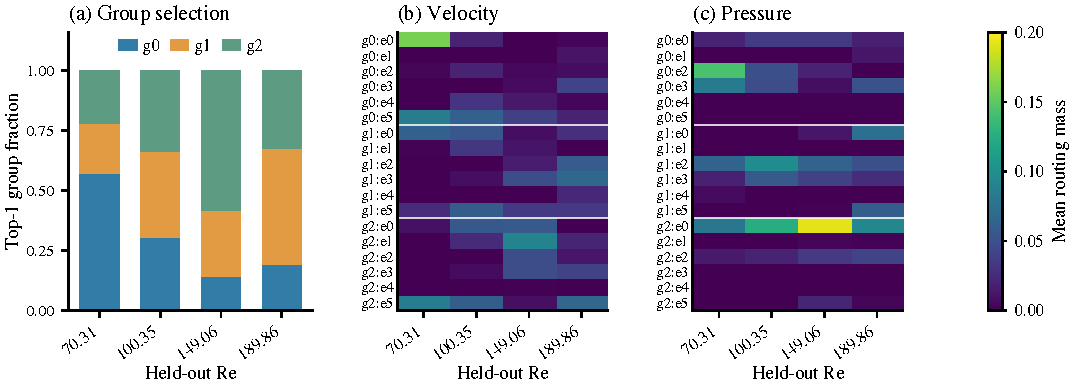
\includegraphics[width=\linewidth]{figures/periodic_internal_routing.pdf}
\caption{
Internal routing of the circular-cylinder Periodic specialist on held-out autonomous rollouts, recorded once per reduced time step at the first integration stage. (a) Top-1 group-selection frequencies. (b,c) Mean routed-expert mass for the velocity and pressure channels. Expert identifiers are local to the corresponding specialist, group, and channel and are not assigned physical labels.
}
\label{fig:periodic_internal_routing}
\end{figure}


\par

\par


\begin{figure}[H]
\centering
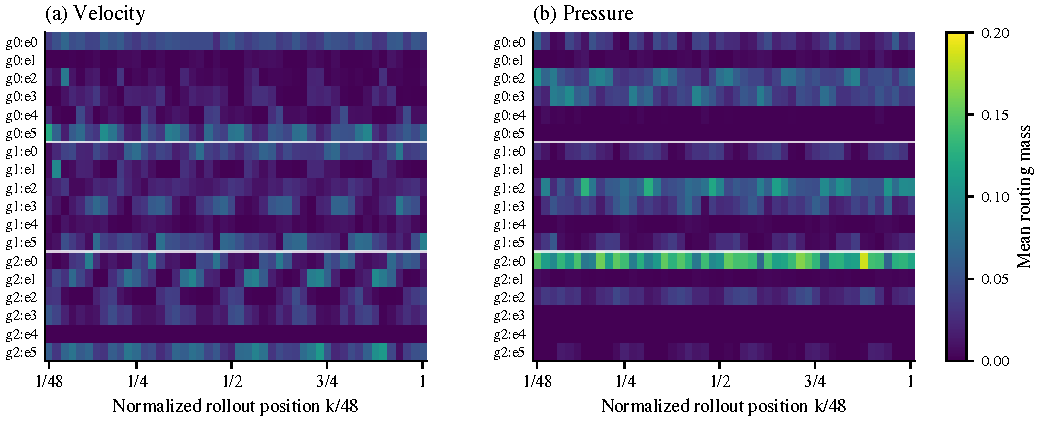
\includegraphics[width=\linewidth]{figures/periodic_rollout_step_routing.pdf}
\caption{
Routed-expert mass versus autonomous rollout position for the circular-cylinder Periodic specialist. Each column averages the routing decision at the corresponding reduced time step over the 52 fixed held-out windows, and all routed experts are retained. The horizontal coordinate is the normalized prediction position $k/48$ and is not interpreted as physical oscillation phase.
}
\label{fig:periodic_routing_step}
\end{figure}


\par

\clearpage
\section{Trainable and active parameter counts}
\label{app:parameter_counts}

\paragraph{Counting convention.}
Total parameters count unique trainable parameters in each analyzed
circular-cylinder specialist. Active parameters count unique trainable
parameters used by one batch-size-one prediction-path routing decision,
not their union across a batch, trajectory, or all RK4 stages. These include
the encoder and refinement blocks, executed routers, the selected group's
shared experts, channel-specific Top-2 velocity and pressure experts, and
the learned pressure correction. Fixed POD bases, projected operators,
normalization statistics, and non-trainable buffers are excluded.

\par


\begin{table}[H]
\centering
\caption{Trainable and per-decision active parameter counts for the analyzed
circular-cylinder specialists. Active counts refer to the sparse prediction
path; counts are exact integers.}
\label{tab:parameter_counts}
\begin{tabular}{lrrr}
\toprule
Specialist & Total trainable & Active prediction & Active fraction \\
\midrule
Hopf & 31,810,392 & 14,165,816 & 44.53\% \\
Periodic & 48,617,547 & 8,308,959 & 17.09\% \\
\bottomrule
\end{tabular}
\end{table}


\par

The Hopf and Periodic specialists activate 44.53\% and 17.09\% of their
trainable parameters per prediction decision, respectively. These counts
describe conditional parameter activation, not measured FLOPs, runtime,
or speedup. Complete parameter-matched counts are unavailable for the
Vanilla-FNN-MoE, DataOnly-MoE, and Global MoE ablations, so the local
architecture comparison is not interpreted as a capacity-matched study.

\paragraph{Native local latency diagnostic.}
For Circular Periodic seed 1248, batch size one and $K=48$, we use three
warm-up runs and ten timed repetitions. The native implementation
includes modal rollout, feature generation, data transfers, algebraic
pressure, all-step physical decoding, and pressure gauge correction.
It excludes physical-history encoding, E2, descriptor construction,
T2-C fusion, model/data loading, and error computation. The Galerkin
NumPy path executes on the CPU; sparse parameter activation does not
imply a proportional wall-clock saving in this implementation.



\begin{table}[H]
\centering
\caption{Local native Circular Periodic diagnostic. GPU memory is peak
allocated bytes. These times are not complete end-to-end latencies.}
\label{tab:local_latency}
\small
\begin{tabular}{@{}lrrr@{}}
\toprule
Model & Median time (s) & GPU peak (bytes) & Time / Dense\\
\midrule
Proposed & 2.1848 & 204,238,336 & 3.32\\
Dense & 0.6579 & 43,111,936 & 1.00\\
Structured & 0.8652 & 43,316,736 & 1.32\\
\bottomrule
\end{tabular}
\end{table}



Matching FOM logs alone does not supply an end-to-end speedup: the same
geometry, physical prediction interval, initialization, and compute/I/O
boundaries must also be measured for the complete ROM pipeline. No such
speedup is claimed here.

\DIFaddbegin \paragraph{\DIFadd{Paired physical-input/physical-output specialist timing.}}
\DIFadd{A separate measurement adds full-size physical-history encoding and
history right-hand-side construction to the original Periodic specialist
(seed 1248). For Circular $Re=70.314635$, the frozen first legal $K=48$
window spans $t=1384.49597$ to $1983.19690$, or 598.70093 physical time
units. Its three-frame physical input is the POD-reconstructed history
on 97,368 points; encoding is timed, but acquiring that history is not.
All 48 velocity and pressure fields are decoded and pressure is
gauge-corrected. The model and inputs are resident before timing.
}

\DIFadd{On an RTX 4090 with a Xeon Platinum 8358P host, with one CPU numerical
thread, batch size one, three warm-ups, ten repetitions, and CUDA
synchronization, the median is 2.18747 s (mean 2.18729 s, sample standard
deviation 0.00462 s; range 2.18034--2.19550 s). The matched production
OpenFOAM log contains 4,692 solver steps and a ClockTime difference of
1,996 s; the largest endpoint discrepancy is $2.3\times10^{-5}$ physical
time units, attributable to stored timestamp precision. The production
solver used one process on a Core i5-14600K VMware host with 16 vCPUs and
at most five concurrent cases. Hardware identification is from the
subsequent source audit, not a contemporaneous benchmark. There is one
FOM timing realization, not ten repeated FOM runs.
}

\DIFadd{The resulting ratio, $1996/2.18747\simeq912.5$, is specifically a historical
production-FOM/warm-specialist wall-time ratio. The FOM interval includes
native solver field writes but excludes meshing, initialization, periodic
detection, and subsequent VTK/NPZ conversion. ROM model/input loading,
output disk writes, E2 selection, and descriptor/T2-C operations are
excluded. Different hardware, concurrency, and I/O boundaries prevent
interpreting this ratio as a hardware-independent or complete hierarchical
pipeline speedup. A fully paired Top-2 end-to-end timing remains unmeasured.
}

\DIFaddend \section{Conditional consistency of output-space fusion}
\label{app:fusion_consistency}
Let $\bm u_\alpha=\alpha\bm u_1+\beta\bm u_2$ and $p_\alpha=\alpha p_1+\beta p_2$, where $\beta=1-\alpha$, $\alpha\in[0,1]$ is constant in space and time over the window, and both candidates share a mesh, parameter, time grid, and pressure gauge. For a common linear operator $D_h$, $D_h\bm u_\alpha=\alpha D_h\bm u_1+\beta D_h\bm u_2$. Thus zero discrete divergence, a zero-mean pressure gauge, and identical affine boundary constraints are preserved only to the extent that both candidates satisfy them.

\paragraph{Nonlinear residuals.}
For a fixed bilinear discretization $N_h$, set $\delta\bm u=\bm u_1-\bm u_2$. Bilinearity gives


\begin{equation}
N_h(\bm u_\alpha,\bm u_\alpha)
=\alpha N_h(\bm u_1,\bm u_1)+\beta N_h(\bm u_2,\bm u_2)
-\alpha\beta N_h(\delta\bm u,\delta\bm u).
\end{equation}


With the sign convention
$R_u(\bm u,p)=\partial_t\bm u-\bm f_h-L_h\bm u+N_h(\bm u,\bm u)+G_hp$, one obtains


\begin{equation}
R_u(\bm u_\alpha,p_\alpha)
=\alpha R_u(\bm u_1,p_1)+\beta R_u(\bm u_2,p_2)
-\alpha\beta N_h(\delta\bm u,\delta\bm u).
\end{equation}


For the pressure residual
$R_p(\bm u,p)=A_hp-[\bm s_0+S_1\bm u+B_p(\bm u,\bm u)]$, with fixed bilinear $B_p$, similarly


\begin{equation}
R_p(\bm u_\alpha,p_\alpha)
=\alpha R_p(\bm u_1,p_1)+\beta R_p(\bm u_2,p_2)
+\alpha\beta B_p(\delta\bm u,\delta\bm u).
\end{equation}


These identities distinguish the candidates' existing residuals from the additional fusion defect. They are conditional algebraic identities, not measurements of the CFD residual: state-dependent limiters or other non-bilinear discretizations require their actual discrete operators.

\paragraph{Energy and phase cancellation.}
For $E(\bm u)=\tfrac12\|\bm u\|_M^2$ with a common positive quadrature matrix,


\begin{equation}
E(\bm u_\alpha)=\alpha E(\bm u_1)+\beta E(\bm u_2)
-\frac{\alpha\beta}{2}\|\bm u_1-\bm u_2\|_M^2.
\end{equation}


Candidate disagreement can therefore reduce the blend's energy relative to the weighted candidate energies, including through phase cancellation. This does not imply that its energy is below the reference solution or below both candidates. Since the blend is not fed back into either specialist, this term is not a recurrent dissipative modification of their reduced dynamics. Empirical residual and phase-sensitive evaluations remain separate from these identities.
\DIFaddbegin 

\subsection{\DIFadd{Measured common-grid diagnostics}}
\label{app:fusion_measured}
\DIFadd{We evaluate both candidates, their frozen T2-C blend, and the common
POD-reconstructed reference on all 16 held-out windows at each square-cylinder
interface ($K=24$, output spacing 4). No window is selected by prediction
quality. These are reconstructed-field diagnostics, not residuals of the
original OpenFOAM finite-volume equations and not errors against unprojected
CFD fields.
}

\paragraph{\DIFadd{Operators and averaging.}}
\DIFadd{On the common 9,400-cell grid, quadratic local least-squares fits define
$D_x,D_y$ and $L$. The initial stencil has 24 nearest cells, with independent
coordinate scaling; it is expanded only if the polynomial matrix is
rank-deficient or has condition number above $10^6$. A 36-neighbor version
checks sensitivity. Actual stencils contain at most 72 cells. Both versions
differentiate a manufactured quadratic polynomial with maximum absolute
error below $1.4\times10^{-10}$. We use
}



{\color{blue}
\begin{equation}
\widehat R_u=\delta_t\bm u+N_D(\bm u,\bm u)+\nabla_Dp-Re^{-1}L\bm u,
\qquad
\widehat R_p=Lp+D_xN_{D,x}+D_yN_{D,y},
\end{equation}
}



\DIFadd{where $N_D(\bm u,\bm u)=uD_x\bm u+vD_y\bm u$.
Residual norms use area-weighted RMS over the interior wake
$6\leq x\leq16$, $1\leq y\leq3$ (2,627 cells).
Centered time differences and summary statistics use output steps 2--23.
The nonzero reference residual includes POD truncation and spatial/temporal
differentiation error; it is not a solver convergence tolerance. Windows
are averaged within each parameter, then parameters equally. The two
parameters per interface each contribute eight overlapping windows;
these windows are not independent experimental replications.
}




{\color{blue}
\begin{table}[H]
\color{blue}\noindent\textbf{ADDED / REPLACEMENT BLOCK}\par
\centering\small
\caption{Measured square-interface diagnostics with the 24-neighbor initial
stencil. Energy error is $|E-E_{\rm ref}|/E_{\rm ref}$ in percent over the
whole domain; residuals are interior RMS. All columns average steps 2--23.
Reference denotes POD-reconstructed CFD, not raw CFD.}
\label{tab:fusion_residual_measured}
\begin{tabular}{@{}llrrr@{}}
\toprule
Interface & Field & Energy error (\%) & $\|\widehat R_u\|$ & $\|\widehat R_p\|$\\
\midrule
S--H & Reference & 0 & 0.00460 & 0.03395\\
& Steady & 2.81100 & 0.00530 & 0.03674\\
& Hopf & 0.14296 & 0.00607 & 0.03513\\
& T2-C & 0.17641 & 0.00520 & 0.03421\\
\midrule
H--P & Reference & 0 & 0.11486 & 0.03736\\
& Periodic & 0.09163 & 0.11627 & 0.03785\\
& Hopf & 0.17298 & 0.11189 & 0.04047\\
& T2-C & 0.05974 & 0.11408 & 0.03631\\
\bottomrule
\end{tabular}
\end{table}
}




\paragraph{\DIFadd{Identities versus measured accuracy.}}
\DIFadd{The maximum absolute discrepancies in the energy, momentum-residual and
pressure-residual identities are $1.2\times10^{-15}$,
$7.4\times10^{-15}$ and $6.1\times10^{-14}$, respectively, across both
stencils and all windows. These values verify the implementation of the
identities, not physical accuracy. The mean blend-energy deficit relative
to reference energy is $0.00314\%$ (S--H) and $0.00181\%$ (H--P), distinct
from the energy-error column in Table~\ref{tab:fusion_residual_measured}.
T2-C has a lower measured pressure residual than either candidate for both
interfaces and both stencils. However, it does not minimize every diagnostic:
the Hopf candidate has a smaller H--P momentum residual and a smaller S--H
energy error. Changing the stencil also changes residual magnitudes
substantially. Thus output blending is not a general residual minimizer,
nor do these results establish discrete conservation or stability.
}

\paragraph{\DIFadd{Phase diagnostics.}}
\DIFadd{A transverse-velocity probe is fixed geometrically at the cell nearest
$(8,2.5)$. We detrend each signal and compare Hilbert phases with the
reference. A window is marked unresolved if the reference dominant
non-Nyquist Fourier component spans fewer than two cycles or its detrended
standard deviation is below $10^{-5}$. None of the 16 S--H windows and only
15 of the 16 H--P windows pass this screening. Even passing this necessary
screen is not evidence that temporal aliasing or Hilbert endpoint effects
are absent. We therefore report phase traces as short-window diagnostics,
not as evidence for a general reduction of phase error or long-time
phase stability.
}




{\color{blue}
\begin{figure}[H]
\color{blue}\noindent\textbf{ADDED / REPLACEMENT BLOCK}\par
\centering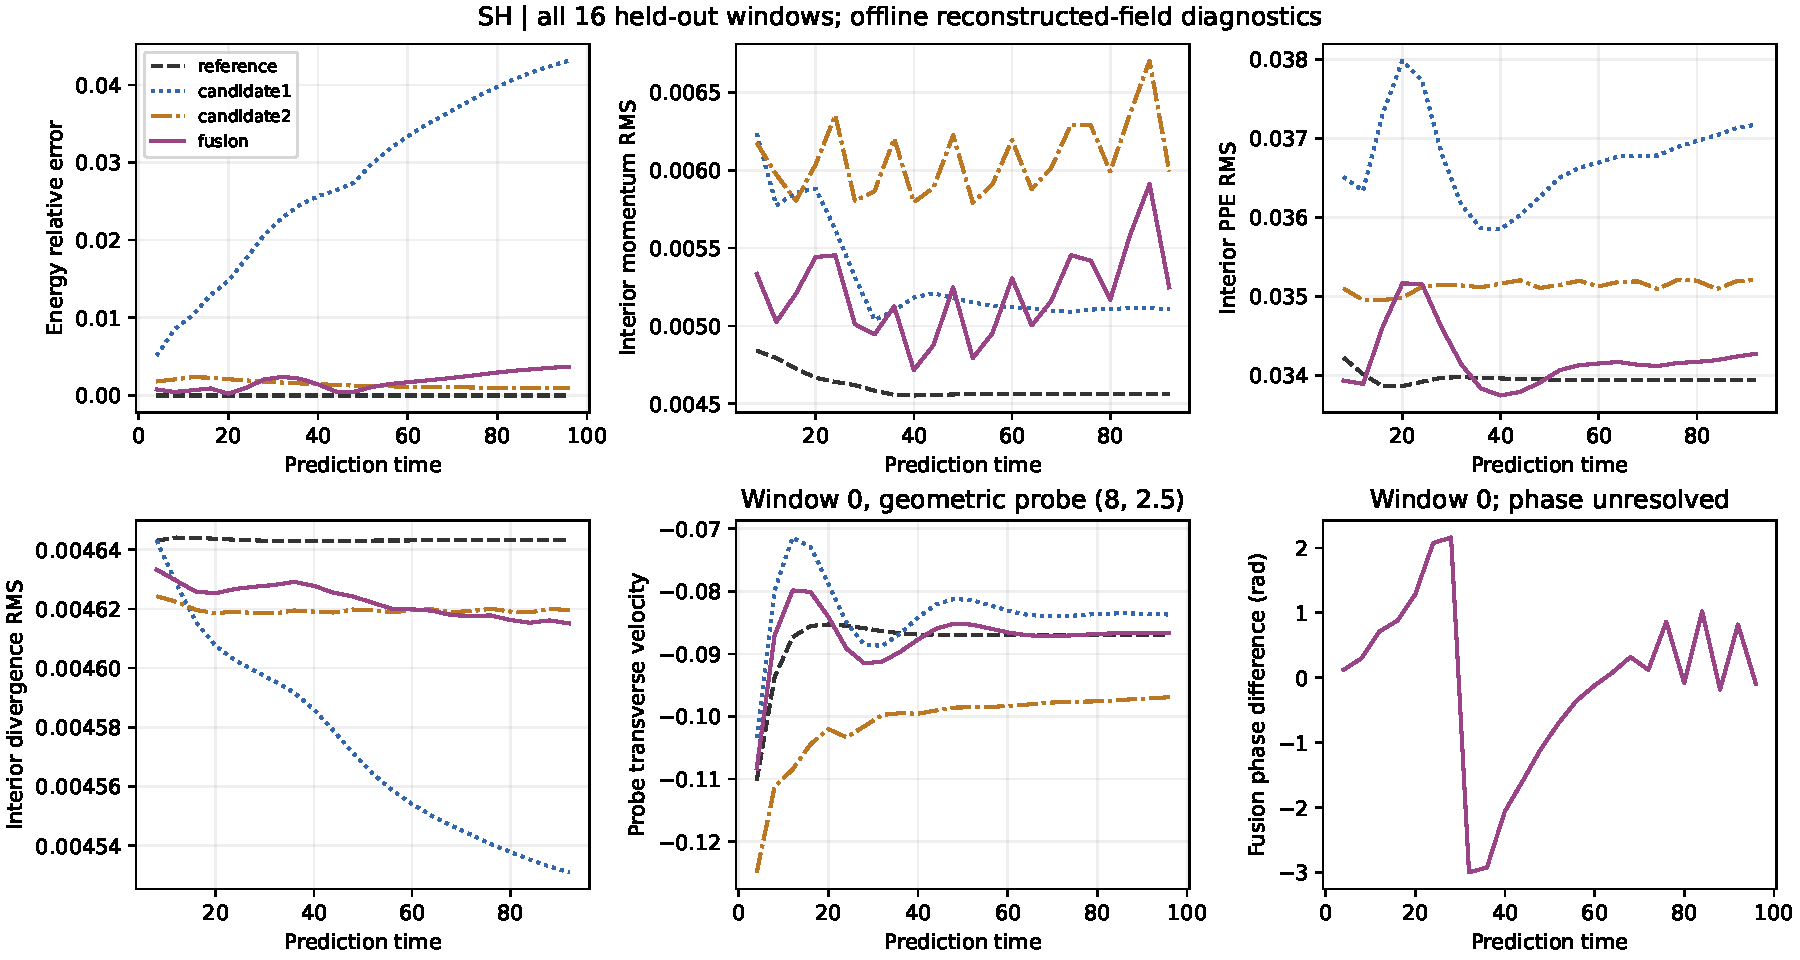
\includegraphics[width=\linewidth]{figures/round3_sh_diagnostics.pdf}
\caption{S--H diagnostics: the first four panels average all 16 windows;
the last two show the first frozen window, not a best-case selection.
Candidate 1 is Steady and candidate 2 is Hopf. Reference is POD-reconstructed
CFD. The unresolved phase trace is descriptive only.}
\end{figure}
}






{\color{blue}
\begin{figure}[H]
\color{blue}\noindent\textbf{ADDED / REPLACEMENT BLOCK}\par
\centering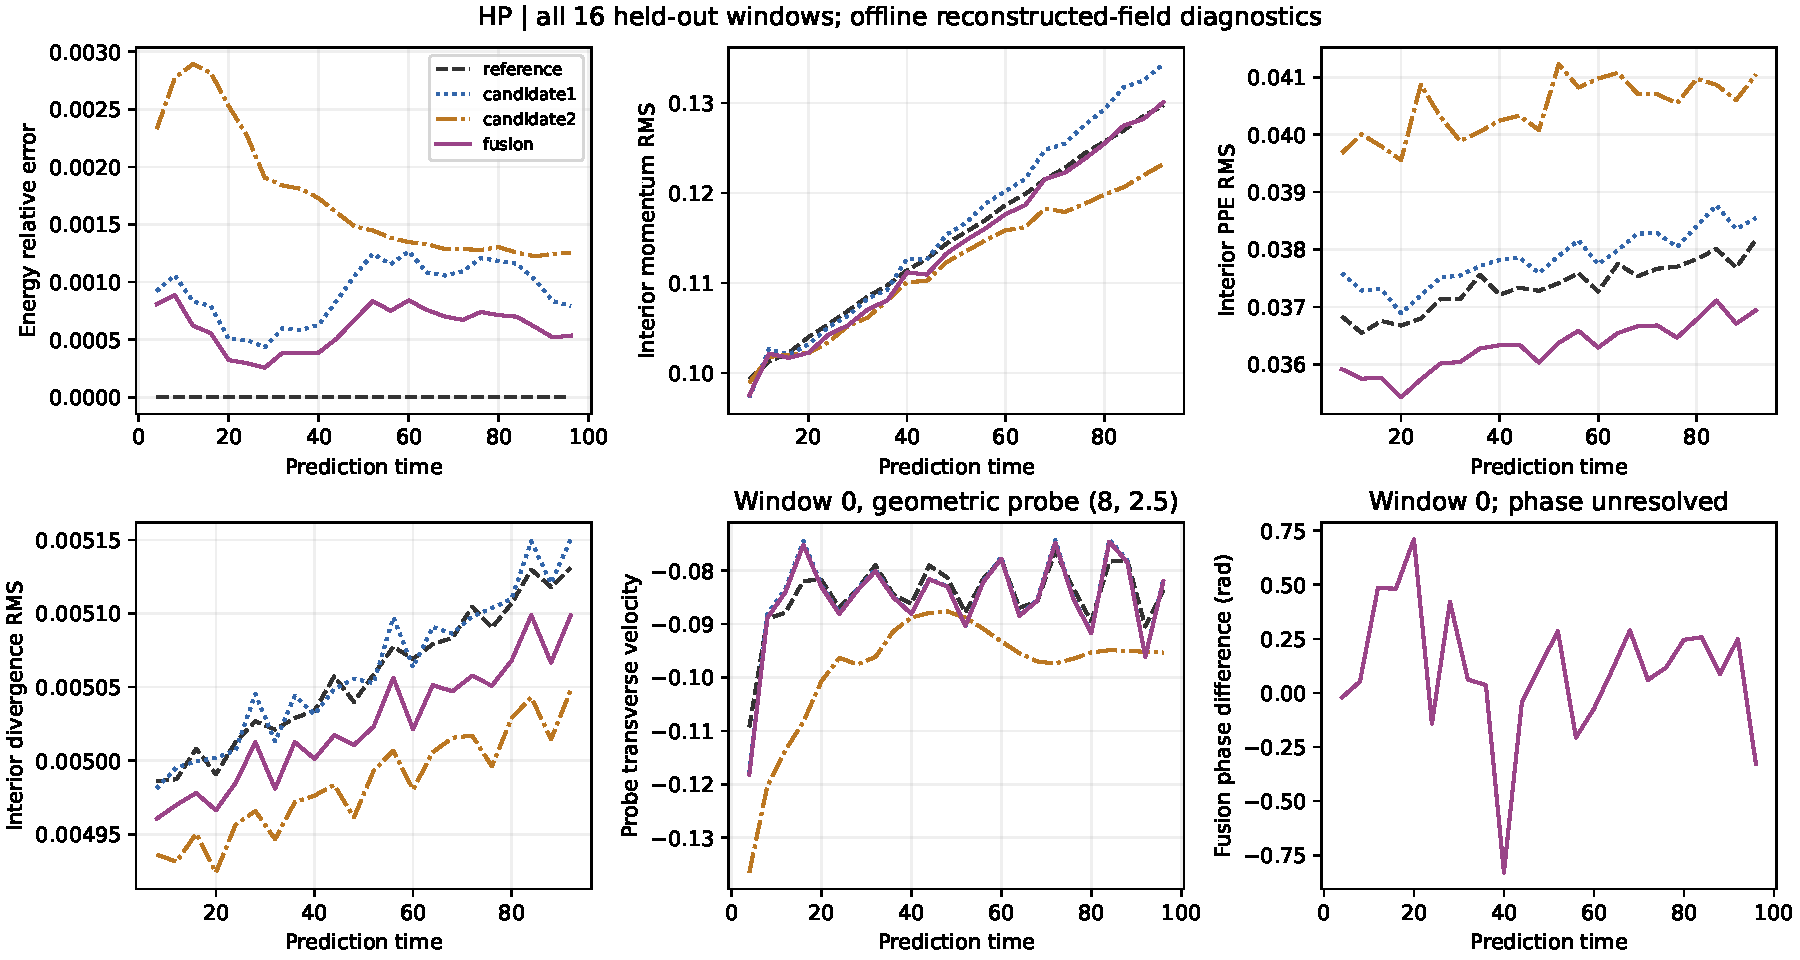
\includegraphics[width=\linewidth]{figures/round3_hp_diagnostics.pdf}
\caption{H--P diagnostics under the same protocol. Candidate 1 is Periodic
and candidate 2 is Hopf. The first four panels average all 16 windows;
the probe and phase panels show the first frozen window, which is
unresolved by the stated phase screen.}
\end{figure}
}






{\color{blue}
\begin{figure}[H]
\color{blue}\noindent\textbf{ADDED / REPLACEMENT BLOCK}\par
\centering
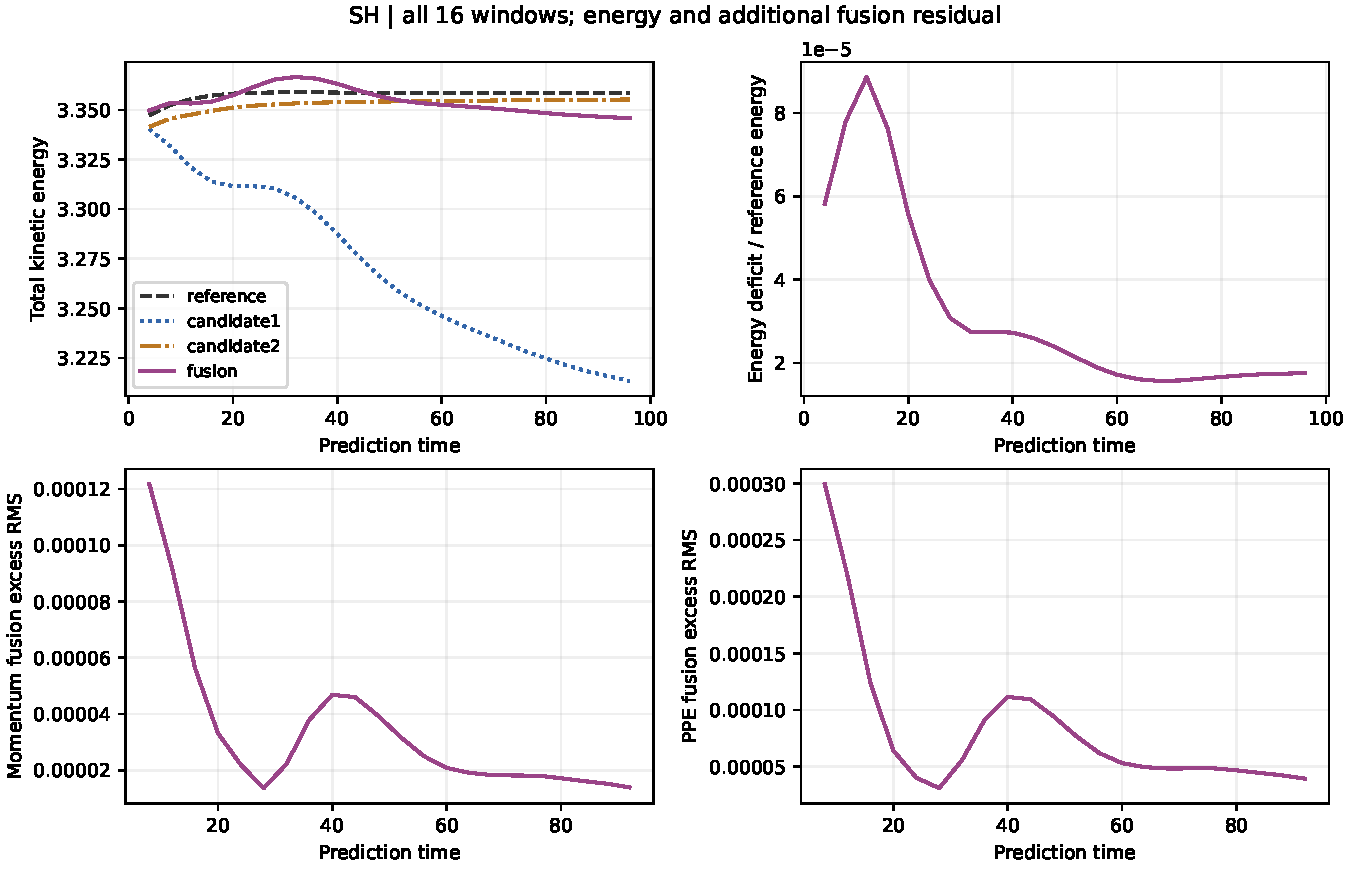
\includegraphics[width=.95\linewidth]{figures/round3_sh_energy_excess.pdf}
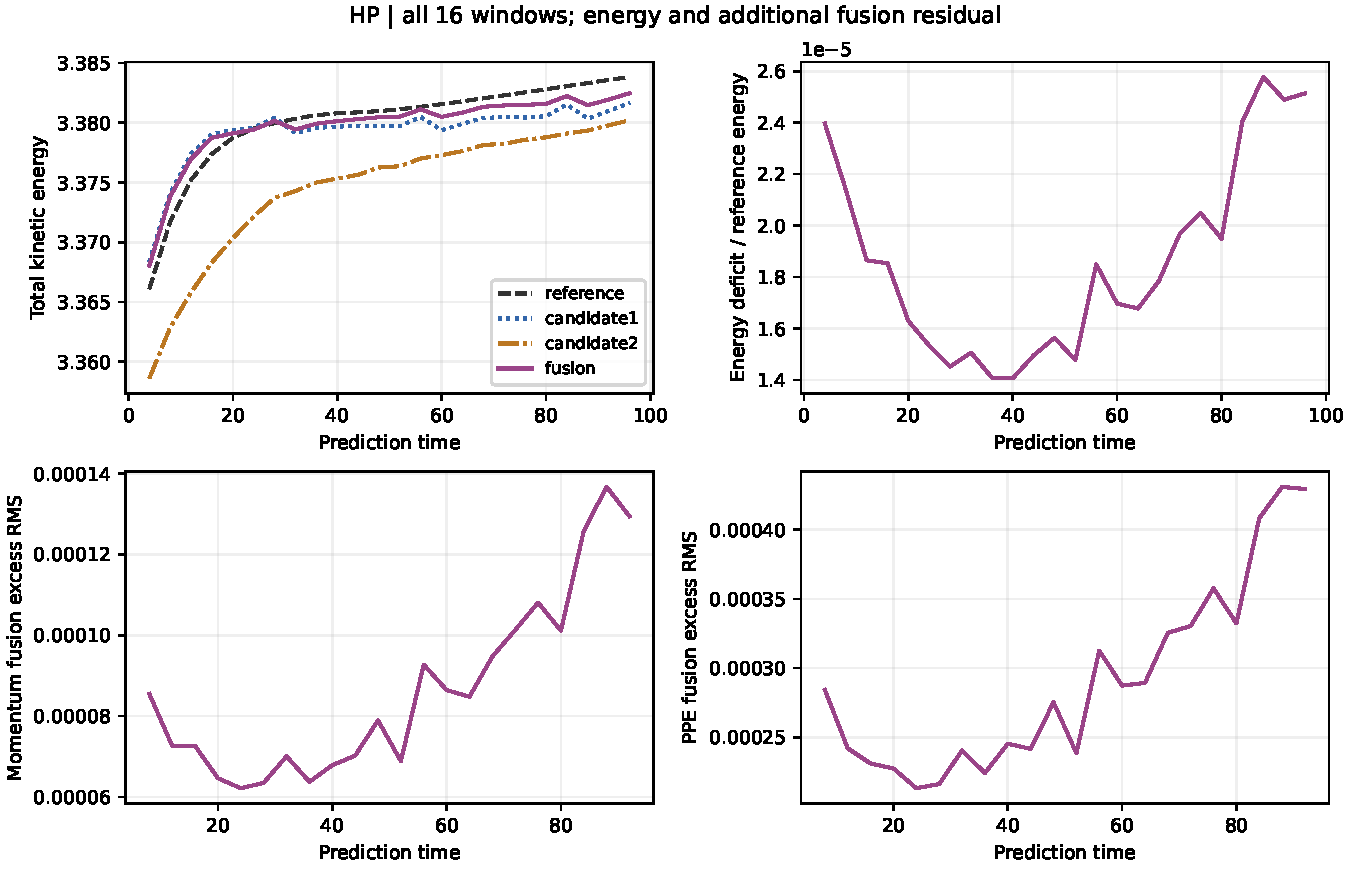
\includegraphics[width=.95\linewidth]{figures/round3_hp_energy_excess.pdf}
\caption{Actual kinetic energy and additional fusion defects averaged over
all windows. The energy deficit is measured relative to the weighted
candidate energies, normalized by reference energy; it is not the energy
error. Momentum and pressure excesses are differences from the
weighted candidate residuals, not the total fused residuals.}
\end{figure}
}
\DIFaddend 




\end{document}
